\section{Introduction}
As discussed in Chapter 1, the attraction effect is a well-studied choice phenomenon where an asymmetrically dominated decoy option increases the choice share of a similar, but superior, target option \parencite{huberAddingAsymmetricallyDominated1982d}. The attraction effect is an example of a context effect, where the relative choice share of an option varies systematically with the choice set.

Though context effects originally were originally demonstrated in preferential choice, recent work has generalized these results to simple, perceptual choice. This result has important theoretical and practical implications for decision-making research. See Chapter 1 for a review of relevant literature on the attraction effect.


\begin{figure}
   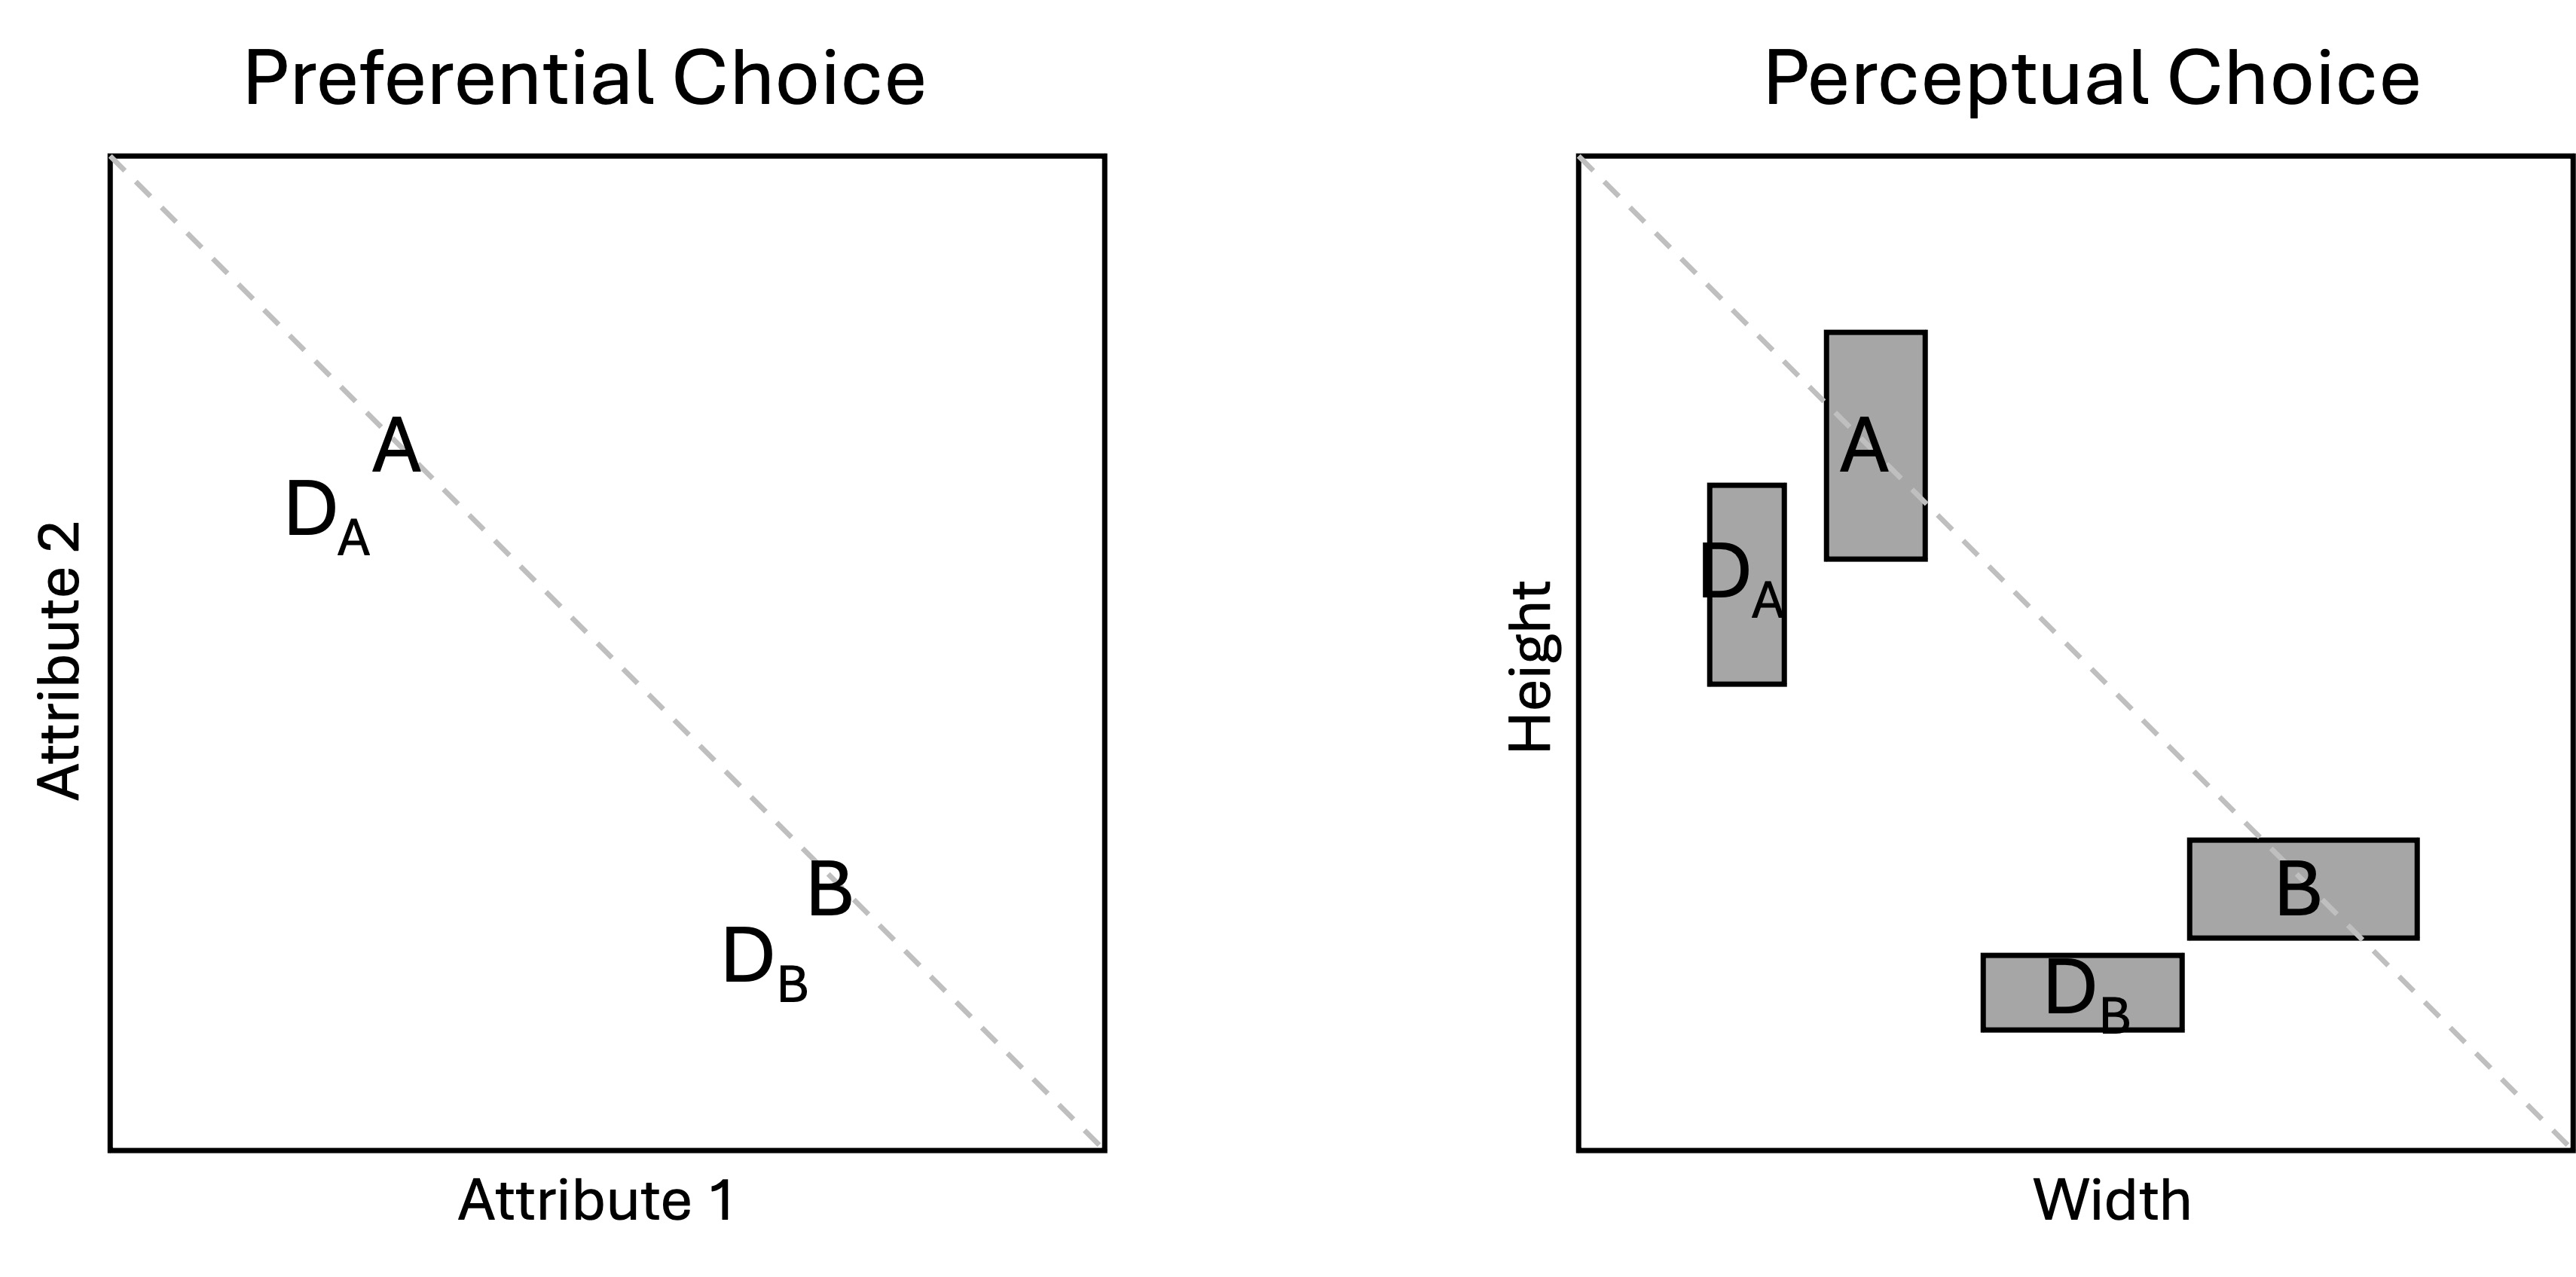
\includegraphics[width=\linewidth]{figures/pref_v_percep.jpg}
   \caption{A graphical depiction of choice options in the attraction/repulsion effect. Left panel: preferential choice. Right panel: perceptual choice.}
   \label{fig:fig_opts}
\end{figure}

Numerous researchers have since demonstrated the attraction effect in preferential choice, including in real-world scenarios. \textcite{doyleRobustnessAsymmetricallyDominated1999} found an attraction effect in real world supermarket choices by adding a decoy option to an existing product set, where the decoy option was the same brand and price as the target, but of a lower volume. \textcite{van2021attract} showed that the attraction effect can be used to induce people to choose healthier food items. \textcite{slaughterDecoyEffectsAttributelevel1999b} showed that the attraction effect can be found even without the explicit attribute descriptions commonly used in laboratory experiments, when participants must infer option attributes. 

% Researchers have demonstrated other context effects, such as the similarity effect, where a similar but equally valuable decoy \textit{decreases} the choice share of a target option \parencite{tverskyEliminationAspectsTheory1972}, and the compromise effect, where an intermediate option decreases the choice share of two relatively extreme options \parencite{simonsonChoiceBasedReasons1989b}. 

% Indeed, other researchers have performed such analyses \parencite{turnerCompetingTheoriesMultialternative2018a,cataldoModelingPreferenceReversals2021,tsetsosPreferenceReversalMultiattribute2010a, molloyWhatResponseTime2019a,berkowitschRigorouslyTestingMultialternative2014b,hotalingTheoreticalDevelopmentsDecision2010,cohen2017multi}, arriving at varying conclusions. 

The attraction effect is not solely limited to consumer choice. Researchers have also demonstrated the attraction effect in risky choice \parencite{mohr2017attraction}, policy choice \parencite{herneDecoyAlternativesPolicy1997b}, intertemporal choice \parencite{mariniAttractionComesMany2020}, probability judgment \parencite{caiWhenAlternativeHypotheses2023}, medical decision-making \parencite{schwartz1999more}, episodic memory judgment \parencite{maylorSimilarityAttractionEffects2007b}, charitable donation \parencite{pittarello2020three},  inference \parencite{truebloodMultialternativeContextEffects2012}, job candidate selection \parencite{highhouseContextDependentSelectionEffects1996}, political choice \parencite{pan1995attractiovoting}, sports prediction \parencite{fang2024context}, and, as will be the focus of much of this dissertation, perceptual choice \parencite{evansImpactPresentationOrder2021,trueblood2013not, trueblood2015fragile, spektorRepulsionEffectPreferential2022,spektorWhenGoodLooks2018b,yearsleyContextEffectsSimilarity2022,turnerCompetingTheoriesMultialternative2018a,liaoInfluenceDistanceDecoy2021}. 


\subsection{From Preferential to Perceptual Choice}

\textcite{choplinComparisoninducedDecoyEffects2005b} and \textcite{yearsleyContextEffectsSimilarity2022} first demonstrated the attraction effects in perceptual choice. In these experiments, participants saw various perceptual stimuli (i.e., ovals, swirled lines, vertical lines) and chose the option most similar to a reference option. The researchers showed that participants were more likely to choose the option paired with a similar (but less similar to the reference stimulus) decoy option.

\textcite{trueblood2013not} also demonstrated the attraction effect in perceptual choice. In their experiments, participants saw three rectangles on each trial, arranged in a horizontal array, and selected the option they perceived to have the largest area. For an example stimulus set, see Figure~\ref{fig:fig_opts} (right panel). Note that options $A$ and $B$ have equal area but trade off in height and width. The decoy options ($D_{A}$ and $D_{B}$, respectively) are smaller in area but are more similar to their respective targets than to their respective competitor. In \textcite{trueblood2013not}'s experiments, participants chose the target option more than the competitor option, on average. 
% \footnote{\textcite{trueblood2013not} also demonstrated the similarity and compromise effects.}. 

Notably, the title of \textcite{trueblood2013not}'s paper was "Not Just for Consumers: Context Effects Are Fundamental to Decision Making", and in their General Discussion, \textcite{trueblood2013not} argued"our experiments suggest that these context effects are a general feature of human choice behavior because they are a fundamental part of decision-making processes. As such, our results challenge explanations of these effects exclusively in terms that are unique to high-level decision making and thus call for a common theoretical explanation that applies across paradigms." (p. 907). According to \textcite{trueblood2013not}, context effects are not idiosyncratic to high-level decision-making but are a fundamental feature of choice. \textcite{trueblood2013not} also used these perceptual results to argue against the context-dependent advantage (CDA) model \parencite{tversky1993context} as well as the Leaky Competing Accumulators (LCA) model \parencite{usherLossAversionInhibition2004a}, as these models use loss aversion  - the idea that an option's disadvantages on an attribute are weighted more strongly than its advantages on other attributes - to account for context effects. \textcite{truebloodMultialternativeContextEffects2012} demonstrated context effects in an inference task and argued similarly against loss aversion.

\textcite{frederickLimitsAttraction2014b} failed to replicate \textcite{trueblood2013not}'s finding of the attraction effect in perceptual choice. \textcite{frederickLimitsAttraction2014b} collected data online, which may have resulted in less precision than a laboratory task, potentially leading to the null finding.

\textcite{turnerCompetingTheoriesMultialternative2018a} replicated \textcite{trueblood2013not}'s results and performed a large scale modeling analysis, comparing the ability of various model mechanisms to account for context effects. For example, \textcite{turnerCompetingTheoriesMultialternative2018a} concluded that pairwise comparisons on individual attributes greatly improves models' ability to account for context effects. This may not be appropriate, however, given a perceptual domain where dimensions may not be separabel. Specifically, in a consumer choice experiment, participants may very well compare options on a single dimension at a time, e.g. comparing cars on their fuel efficiency. However, in a perceptual choice task, it is unlikely that participants are able to separately compare rectangles on the height dimension and on the width dimension and then arrive at an overall judgment. Rather, it is more plausible that participants compare these stimuli holistically.

\textcite{spektorWhenGoodLooks2018b} followed up on this work and demonstrated the \textit{repulsion effect} in a similar perceptual choice experiment. In the repulsion effect, the competitor's choice share is higher than the target's choice share. In \textcite{spektorWhenGoodLooks2018b}'s experiments, the target and competitor options varied in area, such that one option was always larger, though on average they were the same size. The researchers also varied the \textit{target-decoy attribute distance} (TDD), the percentage difference between the target and decoy areas. For example, if TDD is $2\%$, the decoy is $2\%$ smaller than the target. 

\begin{figure}
   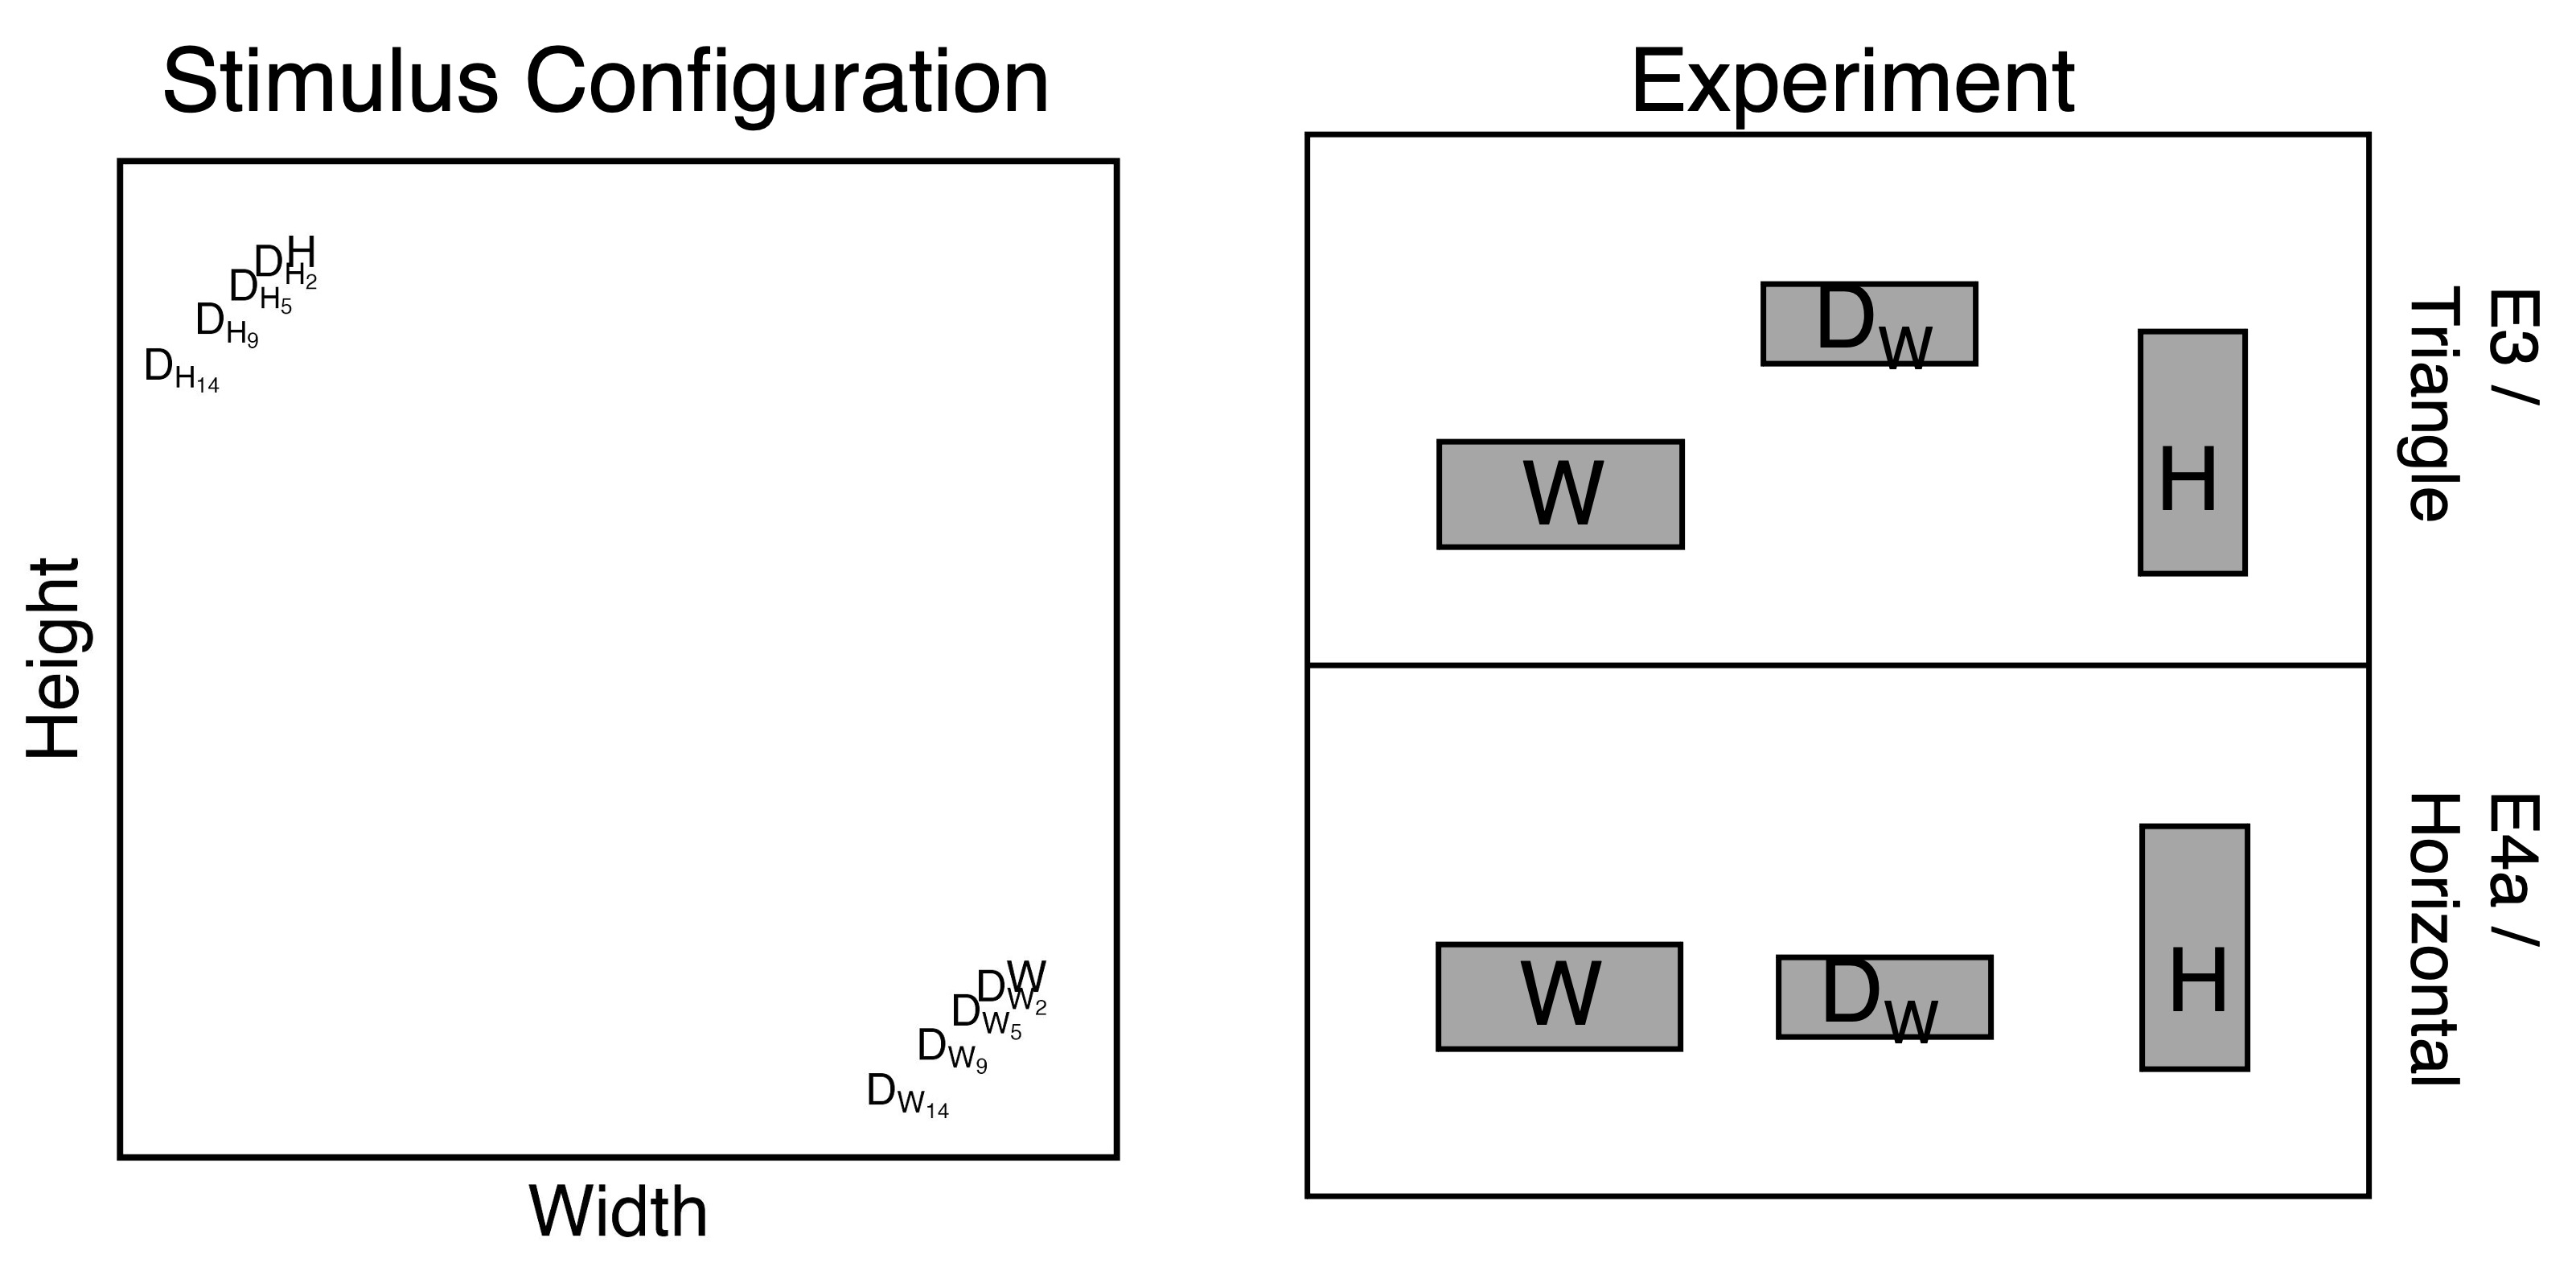
\includegraphics[width=\linewidth]{figures/spektor_stim.png}
   \caption{Stimulus configuration and example trials from \textcite{spektorWhenGoodLooks2018b}, Experiments 3 and 4a. Decoy subscripts indicate TDD. Note that the stimulus in the righthand plot were not shown in the experiment; these are solely for the benefit of the reader.}
   \label{fig:spektor_stim}
\end{figure}

\textcite{spektorWhenGoodLooks2018b} ran a total of five experiments. All experiments showed similar results, so the current focus is on their experiments 3 and 4a, which are the most representative of the article's conclusions. In Experiment 3, the authors varied TDD at four levels: $2\%$, $5\%$, $9\%$, and $14\%$. The rectangles were arranged in a trianglular display on the screen (see Figure~\ref{fig:spektor_stim}, Experiment 3), in contrast to \textcite{trueblood2013not}'s horizontal display. \textcite{spektorWhenGoodLooks2018b} found a repulsion effect, such that the competitor was selected more than the target at all levels of TDD (see Figure~\ref{fig:spektor_data}). 

\textcite{spektorWhenGoodLooks2018b}'s Experiment 4a, however, used the horizontal diplay of \textcite{trueblood2013not} (see Figure~\ref{fig:spektor_stim}, Experiment 4a). Here, they varied TDD at $5\%$, $9\%$, and $14\%$. In Experiment 4a, the data show a slight repulsion effect at low TDD levels that eventually becomes an attraction effect at high TDD levels. 

\textcite{truebloodPhantomDecoyEffect2017c} demonstrated a "phantom decoy" effect in perceptual choice. Phantom decoys are options that are similar to the target, but also superior in value, and are initially presented but made unavailable at the time of choice. They showed that participants chose the target less than the competitor, a result at odds with phantom decoy effects in preferential choice \parencite{pratkanisBriefHistoryResearch1992b,pettiboneExaminingModelsNondominated2000}. 

\begin{figure}
   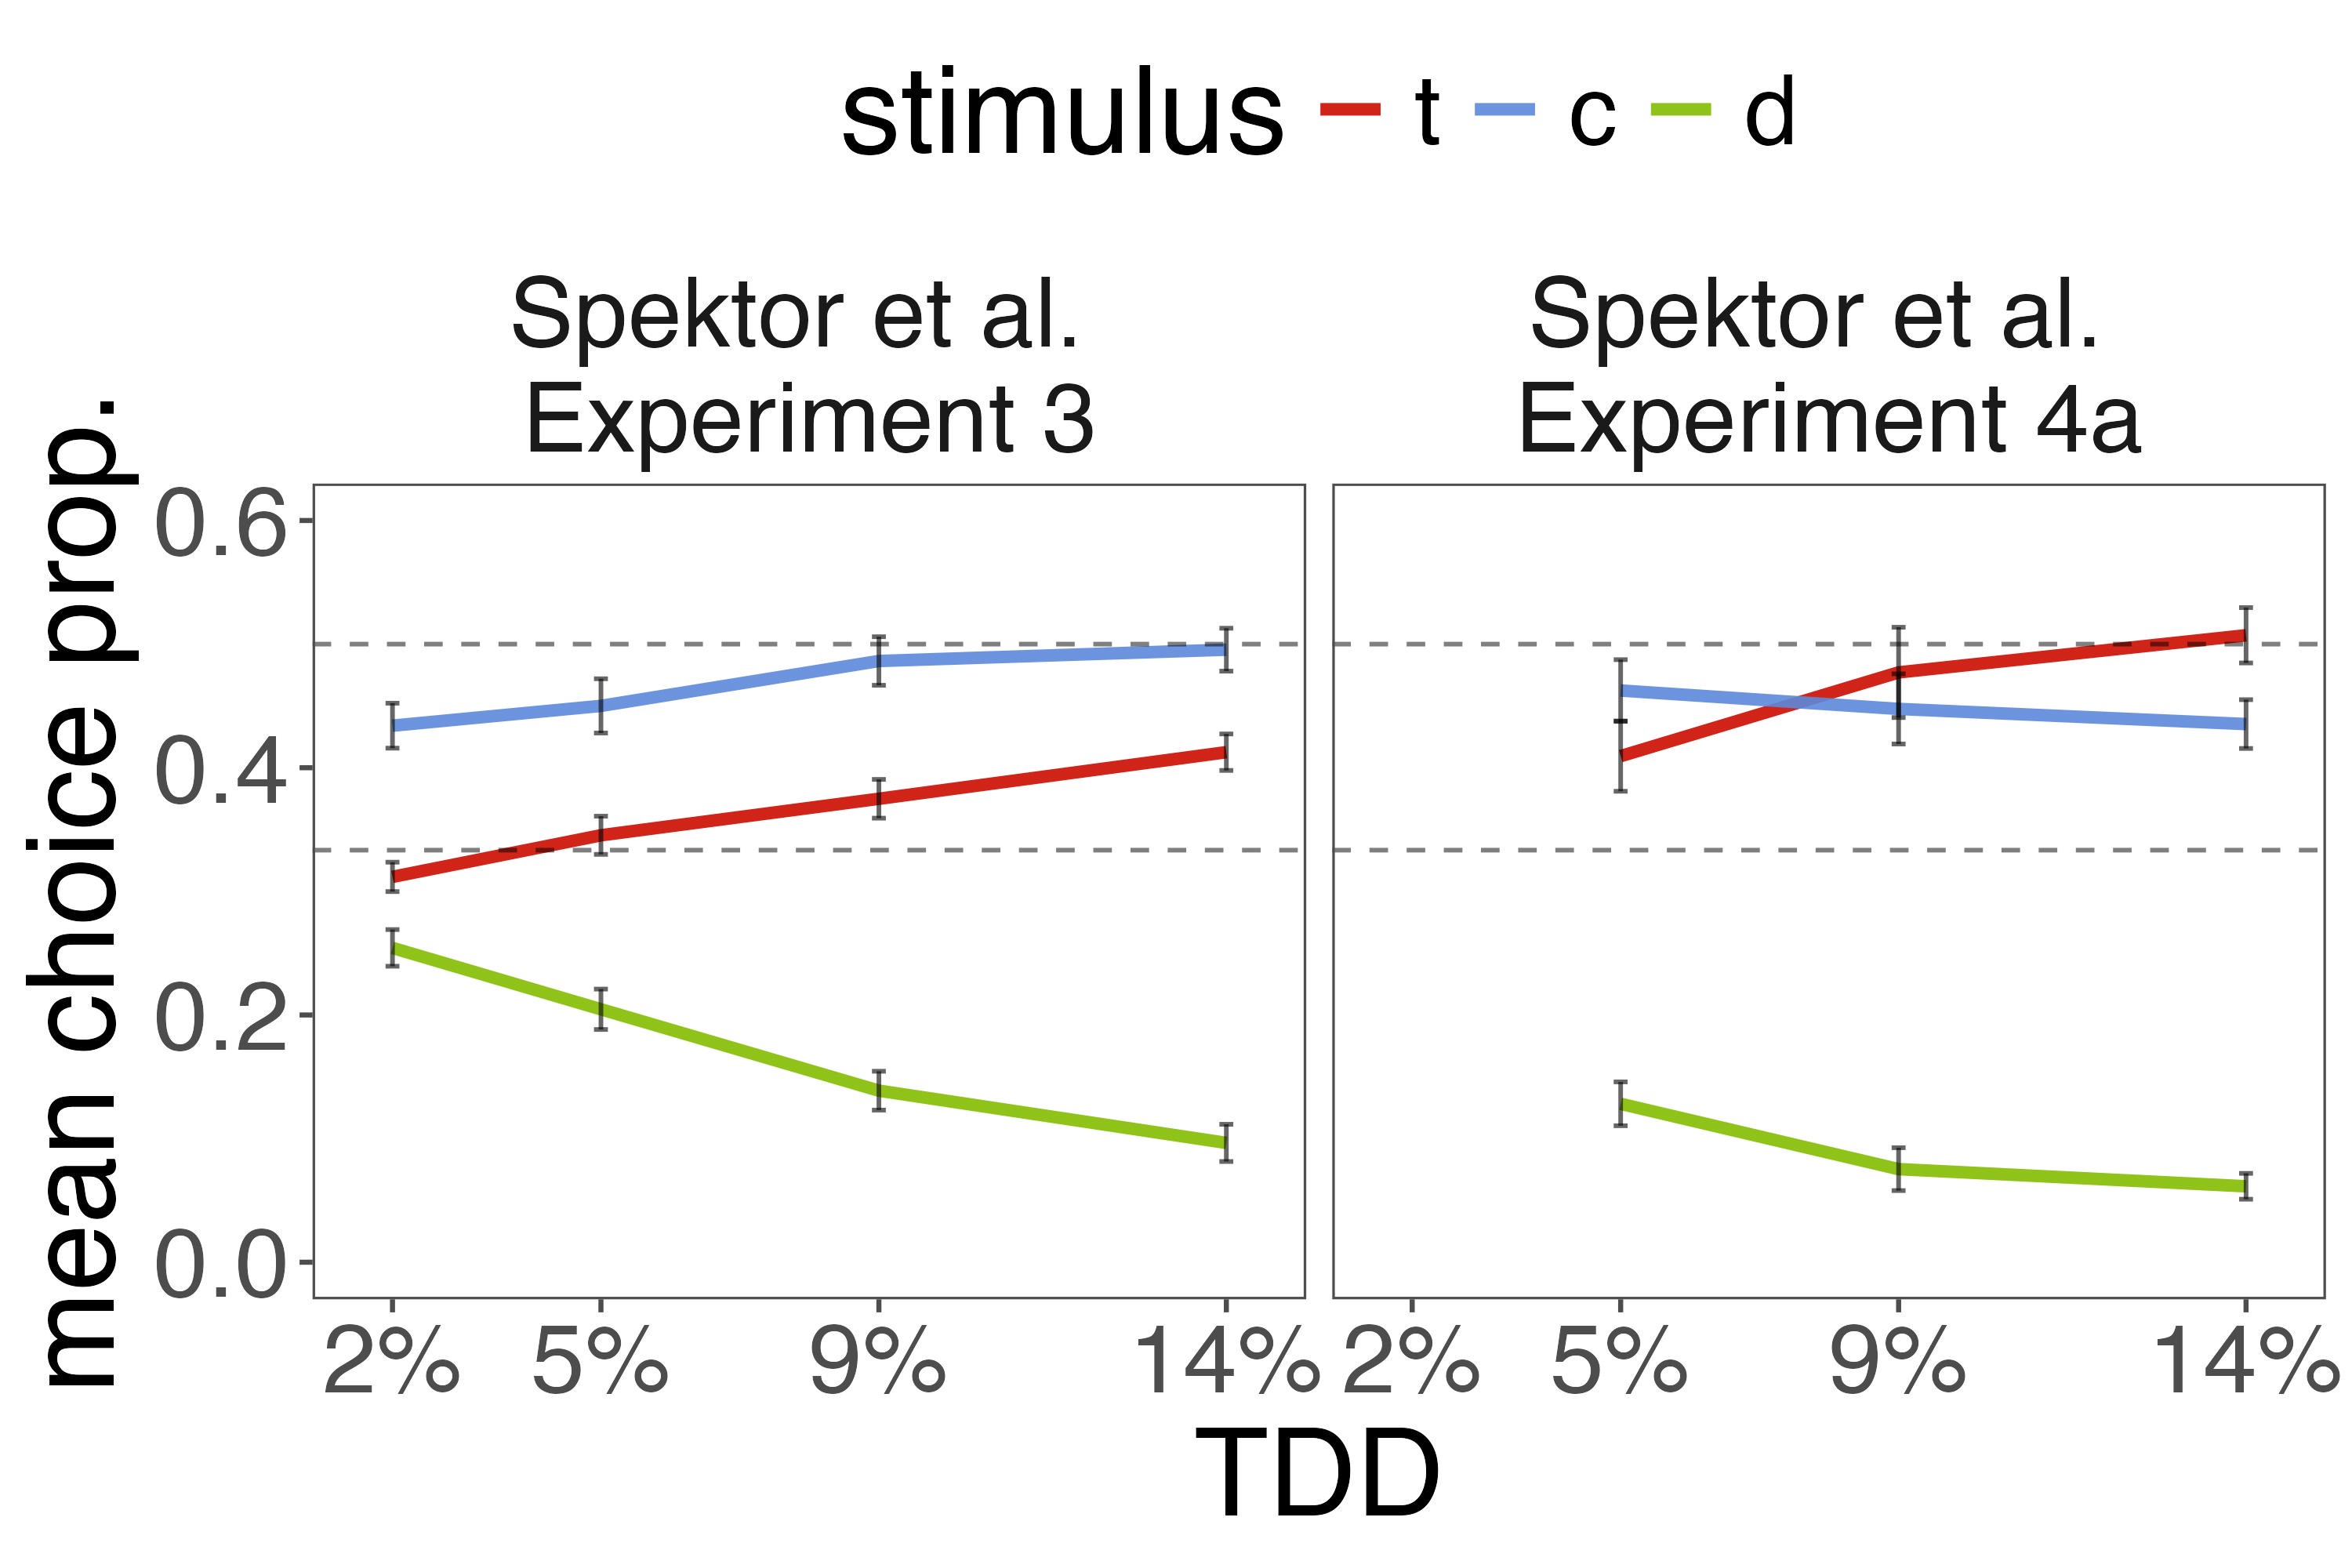
\includegraphics[width=\linewidth]{figures/spektor_data_collapsed.jpeg}
   \caption{Data from \textcite{spektorWhenGoodLooks2018b}, collapsed across choice set. Error bars are $95\%$ CIs of the mean, computed using the within-participants error correction from \textcite{morey2008confidence}. Dashed lines are drawn at .5 and .33.}
   \label{fig:spektor_data} % might consider graphing (or at least writing RSTs) here
\end{figure}

\textcite{liaoInfluenceDistanceDecoy2021} also replicated the general pattern of \textcite{spektorWhenGoodLooks2018b}'s results and also found a an inverse U-shaped relationship between TDD and the attraction effect. Low and high TDD values created a repulsion effect, while intermediate TDD values created an attraction effect. 

\textcite{spektorRepulsionEffectPreferential2022} demonstrated the repulsion effect in both preferential and perceptual choice, using similar stimuli and a similar display configuration to \textcite{spektorWhenGoodLooks2018b} and \textcite{liaoInfluenceDistanceDecoy2021}. Here, the stimuli were squares containing two bars filled to varying degrees with color. In perceptual choice, participants were to select the stimulus with the largest cumulative filled area. In the preferential choice scenario, participants were told that each filled bar represented one possible outcome of a 50-50 gamble, and they were to select the gamble with the highest expected value. Their results were similar to those of \textcite{spektorWhenGoodLooks2018b}, however, where both target and competitor choices increased with TDD.

In a review of the recent context effects literature, \textcite{spektorElusivenessContextEffects2021} identified \textit{attribute concreteness} as a crucial moderating factor on context effects. They defined attribute concreteness as the degree to which observers would agree on the true value of options' attributes. For example, in a preferential choice experiment where attributes are presented numerically, e.g. RAM and Screen Resolution for laptops, attribute concreteness is high. In a perceptual rectangle choice experiment, where observers must rely on their own perception of height and width, attribute concreteness is low. They noted that high attribute concreteness tends to lead to robust context effects while low attribute concreteness has led to mixed results. According to their explanation, the lack of concreteness in perceptual choice is a crucial reason for the varied context effects data. 

Researchers are clearly using perceptual experiments to demonstrate context effects and test theories of choice. These results are clearly informative and theoretically interesting. However, there are distinct differences between these perceptual choice experiments and the preferential choice experiments in which the attraction effect was originally demonstrated. In preferential choice tasks, participants are typically shown a set of options (e.g., laptops, apartments, washing machines), along with the attribute values associated with each option (e.g., 10 GB RAM, 1500 square feet, 2.7 cubic feet capacity). These attributes are typically represented numerically \parencite{hayes2024attribute,banerjeeFactorsThatPromote2024} or with easily discriminable graphical representations \parencite{cataldoComparisonProcessAccount2019b}. The decoy option, therefore, is rarely selected (e.g., $<5\%$ of all trials in many studies), and these selections are assumed to be the result of inattention or accidental responses. Though participants' preferences may be noisy, researchers can generally assume that participants are able to detect the dominance relationship between target and decoy. Perceptual choice tasks, on the other hand, complicate participants' ability to detect this dominance relationship.

In \textcite{spektorWhenGoodLooks2018b}'s experiments, the decoy is selected as often as $25\%$ of all trials in some conditions (see Figure~\ref{fig:spektor_data}), far more often than is common in preferential context effect xperiments. The decoy is also selected less often in experiment 4a (triangle display) than in experiment 3 (horizontal display). Decoy selections also decrease as TDD increases. Finally, though both target and competitor increase in choice share as TDD increases, the target choice share increases at a higher rate than does the competitor, suggesting a strong trade-off between target and decoy choices; stronger, indeed, than the competitor-decoy trade-off. That is, the mean \textit{Relative Choice Share of the Target}, or RST \parencite{berkowitschRigorouslyTestingMultialternative2014b} increases with TDD in both experiments. 

\textcite{spektorWhenGoodLooks2018b} found that a relatively small change in stimulus display (arranging stimuli in a triangle rather than a horizontal line) reverses the attraction effect. Why is it that a relatively subtle change in stimulus display led to a qualitative shift in the data? To answer this question, it is worth considering the differences between \textcite{spektorWhenGoodLooks2018b}'s data and previous context effect experiments. 

Clearly, perceptual discriminability plays a role in \textcite{spektorWhenGoodLooks2018b}'s results. Participants clearly are better able to discriminate the target and competitor from the decoy as TDD increases. Any reasonable account of these data should parse value discriminability from genuine context effects.

Below results from a two-alternative forced-choice experiment show that these stimuli are easily confusable and that the triangle display of \textcite{spektorWhenGoodLooks2018b} decreases discriminability relative to the horizontal display. 

\section{Experiment 1}

The goal of Experiment 1 was to test participants' ability to discriminate between rectangles in the perceptual choice tasks of \textcite{trueblood2013not} and \textcite{spektorWhenGoodLooks2018b}. 
On each trial, participants saw three options (target, competitor, and decoy). After a short delay, two of the rectangles were highlighted and participants chose which of the two rectangles was larger. This two-alternative forced choice (2afc) task allows testing discriminability between all pairs of options. 

This experiment also included a within-participants manipulation to compare discriminability in both the triangle display of \textcite{spektorWhenGoodLooks2018b}, Experiment 3, and the horizontal display of \textcite{spektorWhenGoodLooks2018b} Experiment 4a and \textcite{trueblood2013not}. Otherwise, with a few exceptions discussed below, the experiment followed the stimulus construction and experimental design of \textcite{spektorWhenGoodLooks2018b}, Experiments 3 and 4a. 

\subsection{Methods}

\subsubsection{Participants.}
Data collection took place at the University of Massachusetts Amherst. 86 undergraduate students participated in exchange for course credit. 1 participant who achieved less than $80\%$ accuracy on catch trials (see below) was excluded from all analyses. $1,280$ and $1,296$ trials from the triangle and horizontal conditions, respectively, with response times (RTs) $<100\text{ms}$ or  $>10000\text{ms}$ were also excluded from all analyses, leaving $18,069$ and $18,054$ trials remaining in the triangle and horizontal conditions, respectively. 

\subsubsection{Stimuli.}
Stimuli were gray scale rectangles based on \textcite{trueblood2013not} and \textcite{spektorWhenGoodLooks2018b}. 

Stimuli varied based on trial type. The experiment had two types of trials: critical trials and catch trials.

On each critical trial, the target and competitor had the same area\footnote{Here \textcite{spektorWhenGoodLooks2018b}'s design was simplified as both focal stimuli had the same area.} but differed on orientation, with one stimulus being wide and the other tall. The decoy always had the same orientation as the target. TDD was varied so that the decoy was always $0\%$, $2\%$, $5\%$, $9\%$, or $14\%$ of the target area. Because the target and competitor always had the same area, this means that the decoy was also $0\%$, $2\%$, $5\%$, $9\%$, or $14\%$ of the competitor area. These are the TDD values from \textcite{spektorWhenGoodLooks2018b}, plus a $0\%$ level which acted as a baseline\footnote{When TDD=$0\%$, the target and decoy are identical, so labeling is arbitrary.}.

On each catch trial, there was one large rectangle and two much smaller rectangles. The large rectangle was $260 \pm U(-40, 40) \text{x} 200 \pm U(-40, 40) \text{px}^2$, with a random orientation. The smaller rectangles were $180 \pm U(-40, 40) \text{x} 120 \pm U(-40, 40) \text{px}^2$, one wide and one tall.

\subsubsection{Design.}
There were 5 blocks of trials. In each block there were 60 critical trials, 12 at each TDD level, and 30 catch trials. Of the 12 critical trials at each TDD level, 6 trials were presented in the triangle display and 6 trials were presented in the horizontal display. Finally, 3 of the 6 targets in each display condition at each TDD level were wide and 3 were tall. Of each of these 3 trials, one trial was a target-decoy comparison, one trial was a target-competitor comparison, and one trial was a competitor-decoy comparison. Trial order and rectangle order within each trial were randomized. Thus, this was a $5$ (TDD: $0\%$, $2\%$, $5\%$, $9\%$, $14\%$) x $2$ (display: triangle, horizontal) x $2$ (target-decoy orientation: wide, tall) x $3$ (comparison: target-decoy, target-competitor, competitor-decoy) within-participants design. 

\subsubsection{Procedure.}

On each trial, participants saw three rectangles, labeled 1, 2, and 3 (from left to right). The horizontal distance between all rectangles was constant, but 25 pixels of jitter was added to each rectangle's vertical location. The rectangles appeared for $1825$ms total, but after $500$ms, two of the rectangles changed to a darker shade. Next, all three rectangles disappeared from the screen, and participants were asked to select which of the two darker rectangles had the larger area. The procedure was identical for critical trials and catch trials.

Stimuli were presented on computer monitors with a resolution of 1920 x 1080 pixels. The experiment was programmed in jsPsych \parencite{deleeuwJsPsychJavaScriptLibrary2015}. 

\subsection{Results}

\subsubsection{Catch Trials.}
Participants performed well on the catch trials. The mean percentage correct in the triangle display was $92.6\% (SD=3.77)$, and the mean percentage correct in the horizontal display was $93.2\% (SD=3.52)$. 

\subsubsection{Critical Trials.}
First the baseline TDD level data (TDD=$0\%$) are presented to demonstrate that participants were indifferent between pairs of options when they had identical area. The mean percentage of target choices in target-competitor trials was $48.99\%$ (SD=$10.18$, $95\%$ CI [$46.80$, $51.20$]). The mean percentage of competitor choices in competitor-decoy trials was $49.80\%$ (SD=$11.30$, $95\%$ CI [$47.40$, $52.20$]). The mean percentage of target choices in target-decoy trials was $49.47\%$ (SD=$12.06$, $95\%$ CI [$46.90$, $52.10$]). Participants were indifferent between all pairs of options in the $\text{TDD}=0\%$ trials, so these are not considered further.

Next, the target-competitor trials are presented. Note that in these trials, because both stimuli had the same area, there is no correct response. The results are plotted in Figure~\ref{fig:e1_tc}, with the y axis (arbitrarily) showing the mean proportion of target selections. Though participants were occasionally biased to select either the target or competitor, there was no systematic pattern to their choices, and these data are not discussed further.

\begin{figure}
   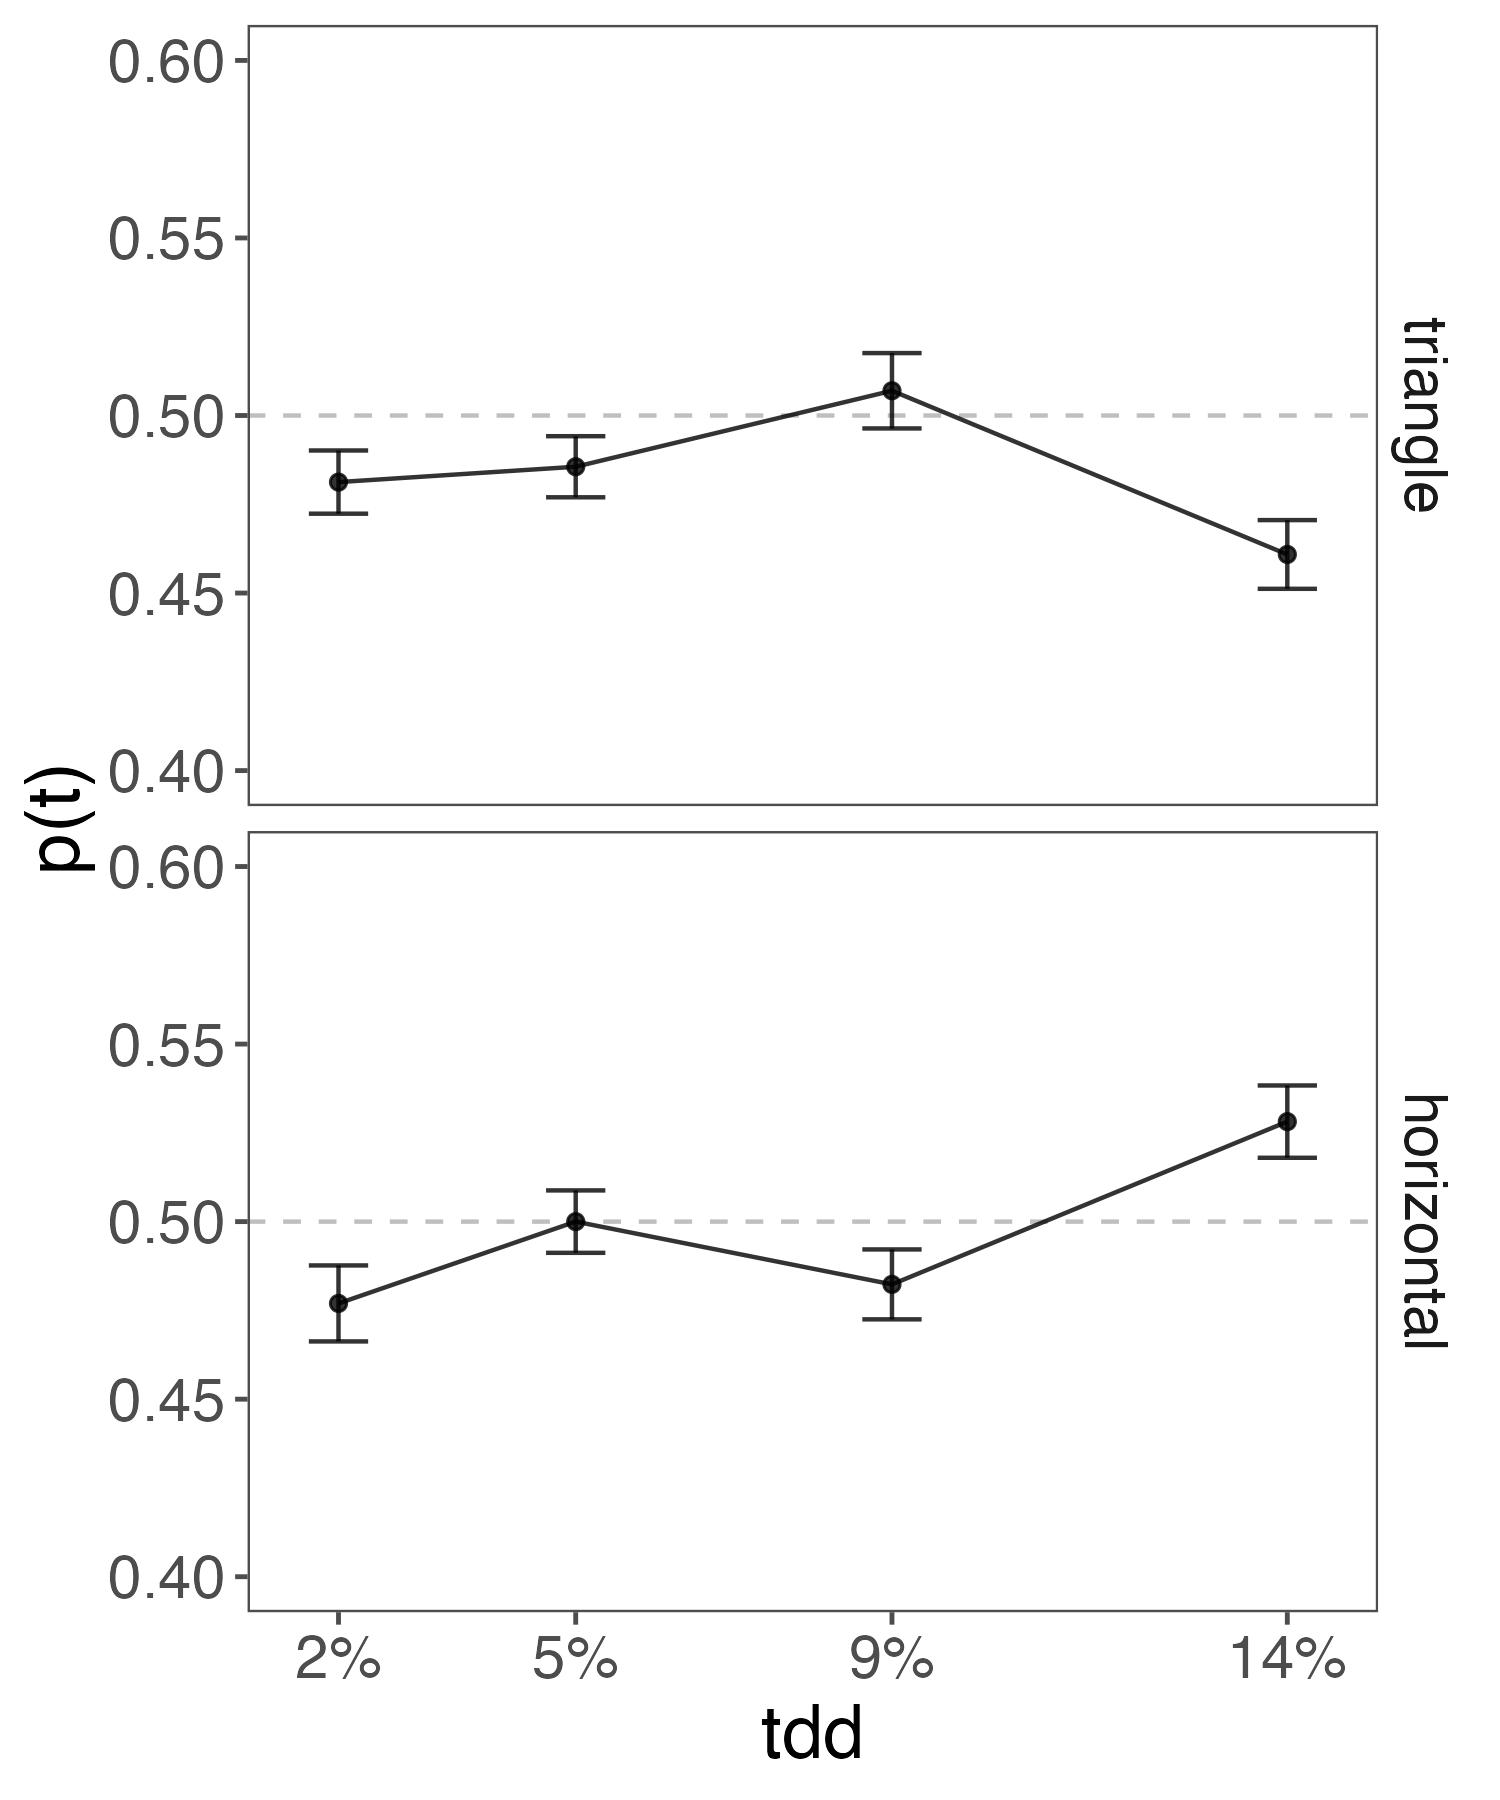
\includegraphics[width=\textwidth]{figures/2afc_tc_choices.jpeg}
   \caption{Experiment 1, mean target choice proportions by stimulus display and TDD for all target-competitor trials. Dashed line is shown at .5.}
   \label{fig:e1_tc}
\end{figure}

The primary analysis was performed on the target-decoy and competitor-decoy trials, excluding all TDD=$0\%$ trials and the target-competitor trials. Note that participants were to select the option with the largest area. Because the target and competitor were always equal in size, and larger than the decoy, a correct response was one in which the decoy was not chosen. 

Mean choice proportions across conditions are shown in Figure~\ref{fig:e1_data}. Participants' performance indeed improves with TDD. Furthermore, their performance is better when stimuli are displayed in the horizontal configuration than in the triangle configuration, and it is also better in target-decoy trials compared to competitor-decoy trials. Finally, there is an interaction, such that as TDD increases, the target-decoy performance is even better than the competitor-decoy performance. See the Appendix for inferential statistics which support these conclusions.

\begin{figure}
   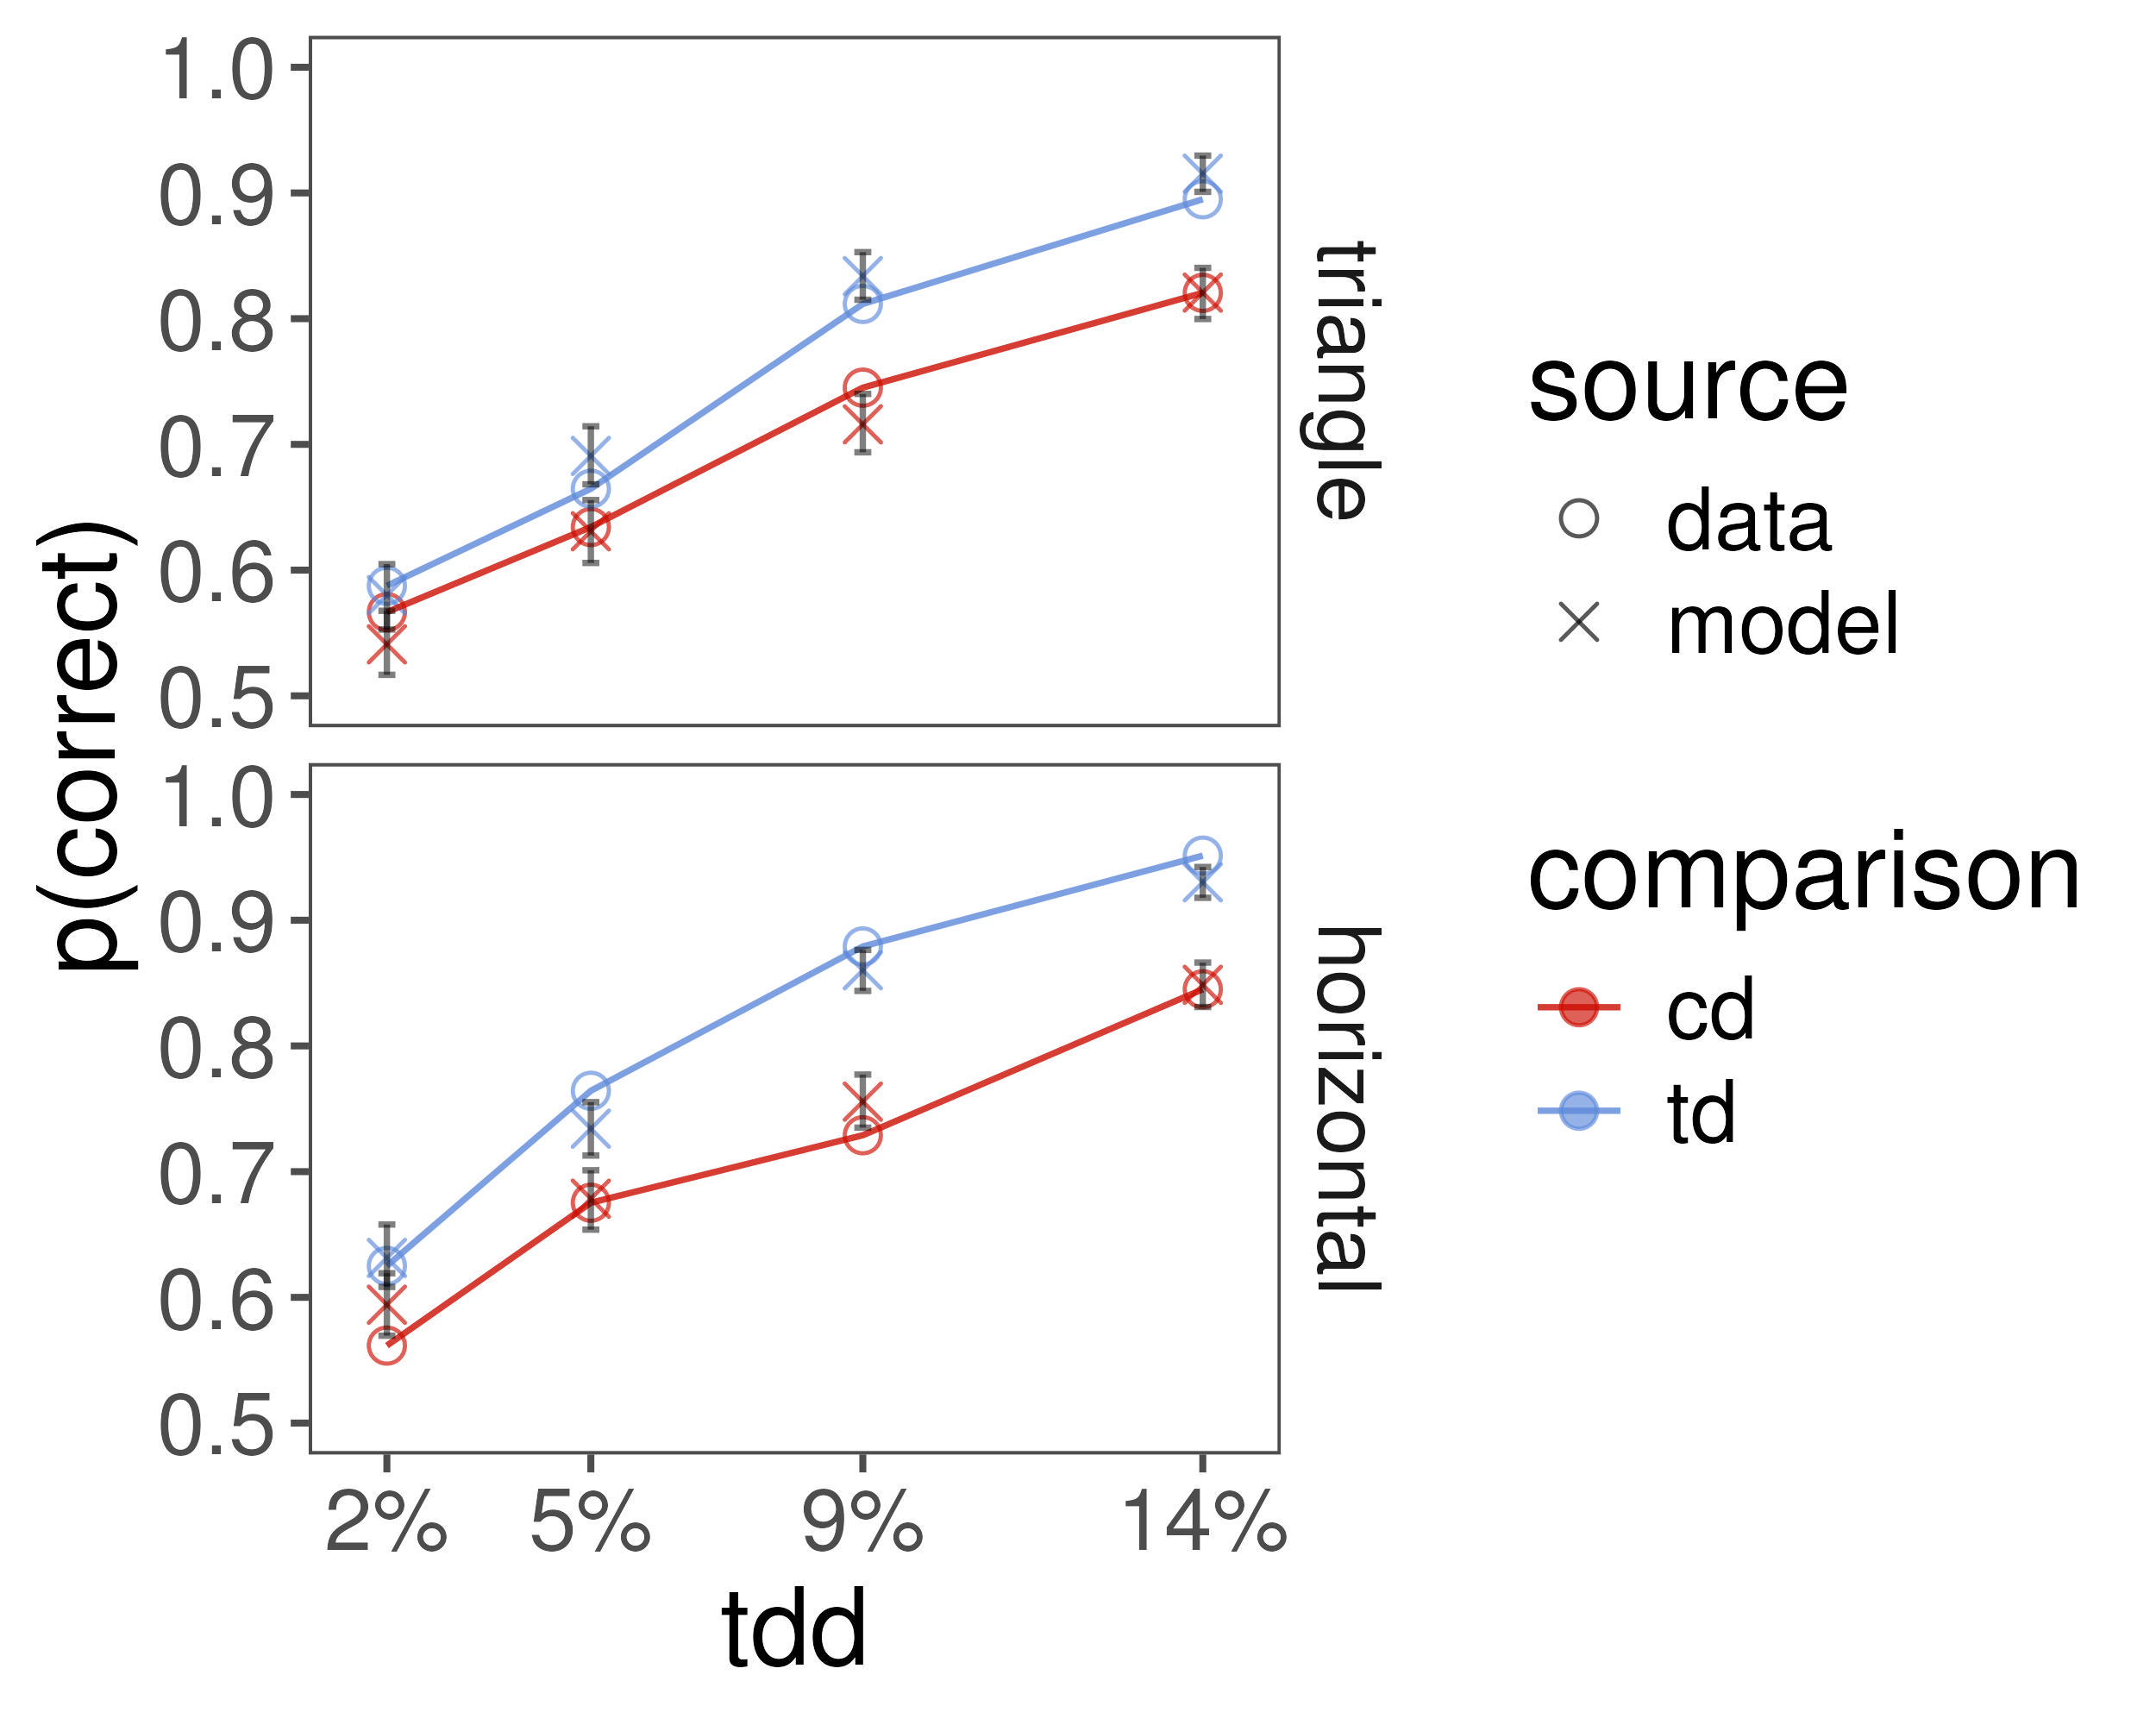
\includegraphics[width=\textwidth]{figures/m14_model_preds_v_data.jpeg}
   \caption{Experiment 1, mean choice proportions by stimulus display, TDD, and comparison. td=target-decoy trials, cd=competitor-decoy trials. Model predictions come from the Bayesian hierarchical logistic regression presented in the Appendix and are presented to demonstrate that the model used for inference adequately fits the data. Error bars are $95\%$ HDIs on the mean.}
   \label{fig:e1_data}
\end{figure}

\subsection{Discussion}

The goal of Experiment 1 was to test participants' ability discriminate between target-decoy and competitor-decoy stimuli in binary perceptual choice. Though participants choose the decoy at non-trivial rates in ternary choice (see Figure~\ref{fig:spektor_data}), previous researchers have not tested participants' binary discriminability. 

Experiment 1 showed that participants are not always able to discriminate between target-decoy and competitor-decoy stimuli. Additionally, this discriminability increases with TDD and that overall discriminability is better in the horizontal compared to the triangle display. Finally, through the interaction of comparison and TDD, it was shown that target-decoy discriminability increases with TDD at a higher rate than competitor-decoy discriminability. 

% It may seem counterintuitive that target-decoy correlations can simultaneously create greater discriminability in binary choice while also generating a repulsion effect in ternary choice. To understand this, it may help to express the correlation $\rho_{TD}$ as:

% \begin{equation}
%    \rho_{TD}=\frac{\mathbb{E}[(X_{T}-\mu_{T})(X_{D}-\mu_{D})]}{\sigma_{T}\sigma_{D}}
%    \label{eqn:rho_expectation}
% \end{equation}

% As $\rho_{TD}$ increases, the difference between sampled target and decoy values converges towards the true difference between $\mu{T}$ and $\mu_{D}$. I also show this by plotting the difference in sampled target and decoy values against increasing values of $\rho_{TD}$.

% \begin{figure}
%    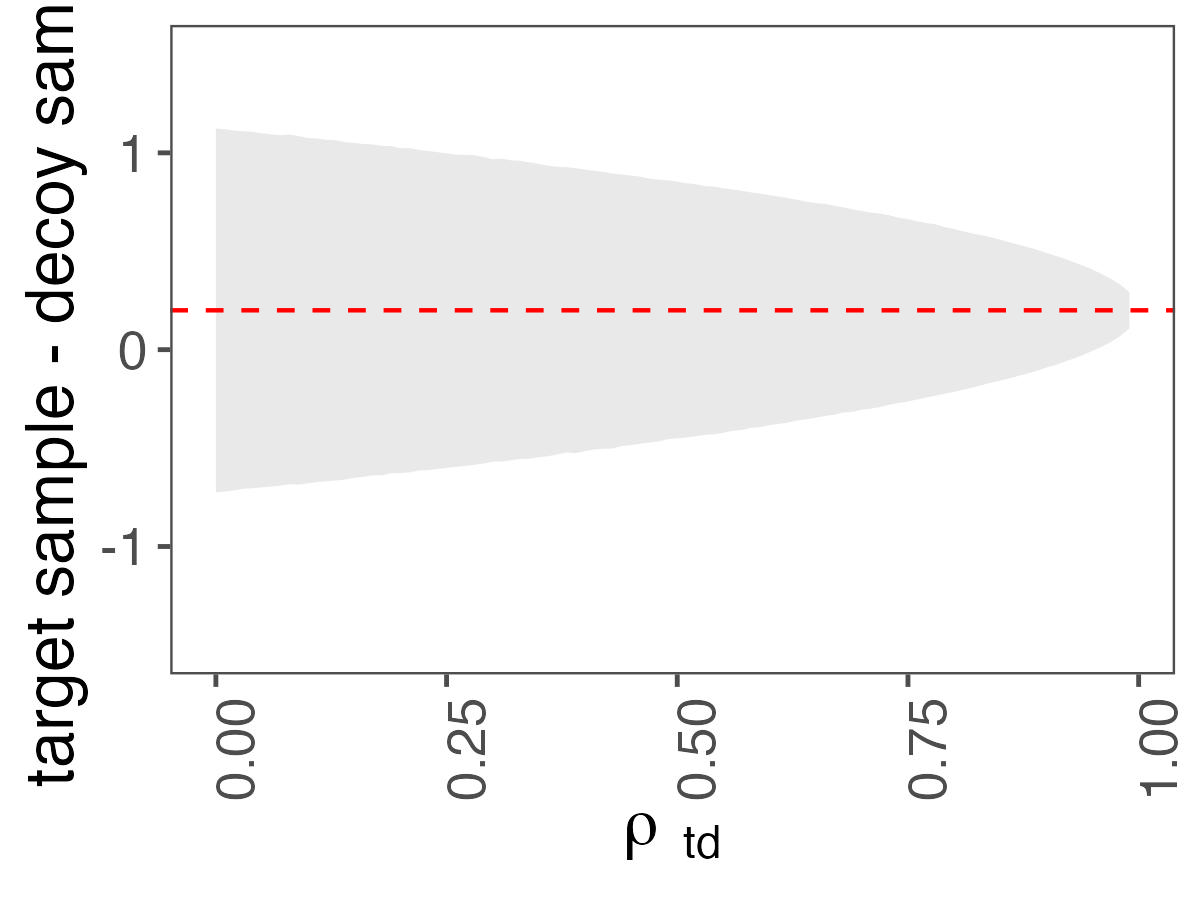
\includegraphics[width=125mm]{figures/sim_mvnorm_vary_r_td.jpeg}
%    \caption{Simulated differences in sampled target minus decoy area (i.e., $X_{T}-X_{D}$) as an plotted against increasing values of $\rho_{TD}$. The lower and upper boundaries of the polygon show the lower and upper quantiles ($2.5\%$ and $97.5\%$, respectively) of the difference between sampled target and decoy values. The dotted red line marks the true $\mu_{T}-\mu_{D}$ value.}
%    \label{fig:sim_mvnorm_vary_r_td}
% \end{figure}

These results are important because they show that target-decoy (and indeed, competitor-decoy) discriminability cannot be taken as a given in perceptual context effect experiments. Researchers must carefully consider how perception of the decoy affects choice. The role of perception is theoretically important because any conclusions about context effects being fundamental to choice \parencite{trueblood2013not} rely on the assumption that context effects are qualitatively similar across choice domains.

In the next section, a Thurstonian perceptual choice model is introduced, with the goal of using it to understand the attraction and repulsion effect. 

\section{Modeling Context-Dependent Perceptual Choice}

\textcite{spektorWhenGoodLooks2018b} argued that their work provides partial evidence in favor of the tainting hypothesis, the idea that decoys sometimes "taint" the value of nearby targets, leading to a repulsion effect. They argued that this is supported by the decrease in competitor choice share as TDD increases. They did note that this high level explanation seems implausible for a perceptual rectangle task.

Another plausible account of \textcite{spektorWhenGoodLooks2018b}'s data is that participants occasionally perceive the decoy to be at least as large as, or larger than, the target. Indeed, the target and decoy are perceptually similar, more so than the decoy and competitor. Their results may be another form of the similarity effect \parencite{tverskyEliminationAspectsTheory1972}, where a similar decoy causes a decrease in the choice share of a target option. Simply put, participants may occasionally select the decoy over target, and they do so more often than they select it over the competitor. This account is consistent with the data shown in Figure~\ref{fig:spektor_data}. As TDD increases, decoy choices decrease while target choices increase. Though competitor choices also increases with TDD, the target choice shares increase at a higher rate. There appears to be a strong tradeoff between target choices and decoy choices. This explanation is, however, distinct from theoretical accounts of the attraction effect. \textcite{spektorWhenGoodLooks2018b} dismiss such an account because the target was always chosen more often the decoy. This does not, however, rule out that possibility that, on the trials where the decoy was chosen, it was more likely to be chosen over the target than the competitor. In other words, participants do not always select the decoy; however, when they do, they more often select it over the similar target than the dissimilar competitor. 

One goal of this work is to separate the role of perceptual and decisonal processes in context effects. To do so, we begin with an extreme stance - that such experiments are solely perceptual experiments rather than decision-making experiments and that no high level decision processes are occurring. This extreme assumption is quite likely incorrect, but it may be helpful in understanding existing data. For example, if a perceptual model can account for the repulsion effect without incorporating higher-level decision processes, (such as loss aversion or attribute weighting, as invoked by some cognitive models of context effects), this provides evidence that the repulsion effect is not a decision-making phenomenon, but a perceptual one. On the other hand, if perceptual processes explain part, but not all, of the repulsion effect, this provides evidence that higher-level decision processes must be invoked in a complete theoretical account of these data.

There is a large body of psychological research, beginning with the work of \textcite{thurstone1927law}, which treats the stimulus perception as a random variable. In his famous "Law of Comparative Judgment" paper, \textcite{thurstone1927law} showed that researchers can use binary choice proportions to estimate the psychological distance between stimuli, by treating perceptual intensity as a Gaussian random variable. According to Thurstone's models, given a proportion of the trials on which participants were able to discriminate between two stimuli, researchers can estimate the average psychological distance between these perceptions, scaled by their standard deviations. Thurstone considered multiple forms of this model, but the most relevant model is his Case $II$ model, which allows for correlations between perceptions. Models of this class are often called \textit{Thurstonian}.

Thurstone's work has been particularly influential on the choice modeling literature. In marketing and economics, researchers treat the utilities of choice options as random variables, which are often assumed to be Gaussian or Extreme Value Distributed and estimate choice models known as Random Utility Models (RUMs) \parencite{mcfadden2001economic,hausman1978conditional,train2009discrete}. Often, though not necessarily, these models share the common property that value - be it the utility of a consumer product, the perception of magnitude in a perceptual task, or memory signal in a recognition task - is stochastic while choice is deterministic  (c.f. \textcite{benjamin2009signal}).

Based on this research, we consider the Thurstonian choice model which will be applied to perceptual choice. This model treats the experiments of \textcite{trueblood2013not} and \textcite{spektorWhenGoodLooks2018b} as perceptual tasks, rather than decision tasks. This assumption may be incorrect, but the extent to which it can explain existing data can still be highly informative. According to this model, the perceived areas of each rectangle on each trial are sampled from an underlying multivariate probility distribution. Participants then deterministically choose the option with the largest perceived area. Thus, while perception is stochastic, choice is deterministic.

\subsection{A Thurstonian Choice Model}

In a perceptual choice task such as that of \textcite{spektorWhenGoodLooks2018b}, the value/utility of each option is its perceived area. According to the model, on each trial $i$ with choice set $K$, the perception $\mathbf{X_i}$ of all $3$ stimuli is sampled from a multivariate Gaussian distribution:

\begin{align}
   \mathbf{X}_{i} \sim \mathcal{N}(\boldsymbol{\mu}, \boldsymbol{\Sigma})
   \label{eqn:mvnorm}
\end{align}

where $\boldsymbol{\mu}$ is the column vector:
\begin{align}
   \begin{pmatrix}
      \mu_{T} \\
      \mu_{C} \\
      \mu_{D}
      \end{pmatrix}
   \label{eqn:mu}
\end{align}

where the subscripts $T$, $C$, and $D$ indicate target, competitor, and decoy, respectively.

$\boldsymbol{\Sigma}$ is a positive semi-definite $3 \text{x} 3$ covariance matrix computed by:

\begin{align}
   \boldsymbol{\Sigma}=S\boldsymbol{\Omega}S
   \label{eqn:Sigma}
\end{align}

where $S$ is a diagonal matrix consisting of: 

\begin{align}
   \begin{pmatrix}
      \sigma_{T} & 0 & 0 \\
      0 & \sigma_{C} & 0 \\
      0 & 0 & \sigma_{D} 
   \end{pmatrix}
\label{eqn:S}
\end{align}

with $\sigma_{T}$, $\sigma_{C}$, $\sigma_{D}$ denoting the standard deviations for target, competitor, and decoy, respectively. These parameters reflect the extent to which area perception varies from trial to trial for each stimulus type. $\boldsymbol{\Omega}$ is a $3\text{x}3$ correlation matrix:

\begin{align}
   \begin{pmatrix}
      1 & \rho_{TC} & \rho_{TD} \\
      \rho_{TC} & 1 & \rho_{CD} \\
      \rho_{TD} & \rho_{CD} & 1 
   \end{pmatrix}
\label{eqn:O}
\end{align}
with $\rho_{TD}$, for example, denoting correlation between target and decoy perception. These parameters measure the extent to which area perceptions "move" together for certain pairs of stimuli. For example, as will be shown below, the target and decoy perceptions are strongly positively correlated, meaning that on trials where the target is perceived to be relatively large, the decoy will also tend to be perceived relatively large.

As mentioned above, the model assumes that value is stochastic while choice is deterministic\footnote{This also assumes ties are not possible, which is true if and only if perceived area is absolutely continuous.}. The model always chooses the option perceived as largest, regardless of the magnitude of the difference between the "winner" and "runners-up". That is, given a vector $\mathbf{X}_i$ of perceived areas on trial $i$ with set $K$, the probability a participant selects stimulus $j$ as largest is:

\begin{align}
   P(j|i,K)=P(\mathbf{X}_{ij}>\mathbf{X}_{ik}), \forall k \in K, j \neq k
   \label{eqn:pchoice}
\end{align}

If all correlations $=0$ and $\sigma_{T}=\sigma_{C}=\sigma_{D}$, the model collapses to a trivariate version of the standard Thurstonian Case V model \parencite{thurstone1927law} often used by cognitive psychology researchers. Models of this form have closed form solutions and their predictions are easy to compute.

On the other hand, if any correlations are non-zero, the closed form solution of this model does not exist, and to compute predictions and estimate model parameters, researchers must use simulation or numerical integration methods \parencite{train2009discrete}. 

This model is easily capable of generating a(n) attraction (repulsion) effect by assuming $\mu_{T}>\mu_{C}$ ($\mu_{C}>\mu_{T}$), i.e., that on average target and competitor stimuli differ in their perceived areas. This is an ad hoc assumption that may describe the data well but will generate limited theoretical insight. 
% Moreover, I wil later present empirical data that suggest, generally speaking, $\mu_{T}\approx\mu_{C}$. 

On the other hand, the correlations between perceived area, may allow the model to predict context effects. Other researchers have considered correlations in RUMs as a mechanism for context effects. \textcite{kamakura1984predicting} argued that the correlation between a pair of options in the multinomial probit model reflect their similarity, or substitutability. They implemented a model where the correlation between options is parameterized as a decreasing function of their distance in attribute space. They showed, via simulations, that this model is able to successfully predict the similarity effect. They also fitted the data to risky choice data, which were collected using stimuli designed to elicit the similarity effect, and found that the fitted model could successfully account for the data. 

\textcite{natenzon2019random} implemented a Bayesian probit model, in which participants are assumed to sample from a multivariate normal distribution on each trial, with the correlation between options being related to their similarity in multiattribute space. \textcite{natenzon2019random} also suggested that similarity is related to ease of comparability. They fitted the model to frog mating choice data and showed that not only can the model explain choice reversals (i.e., context effects), but the estimated correlations between pairs of options were greater for options closer in multiattribute space. 

It is worthwhile considering then, the role of correlations (i.e., $\rho_{TC}$, $\rho_{TD}$, and $\rho_{CD}$) in predicting the attraction and repulsion effects in perceptual choice. 

$\rho_{TD}$ and $\rho_{TC}$ were varied from -1 to 1; in other words, all rectangles oriented the same way (i.e., target and decoy) shared one correlation and those oriented differently (i.e., target and competitor, decoy and competitor) shared another correlation. These model predictions are shown in Figure~\ref{fig:3d_model}. It was assumed that $\mu_{T}=\mu_{C}>\mu_{D}$ and that $\sigma_{T}=\sigma_{C}=\sigma_{D}$\footnote{Experiment 2 presents evidence supporting these assumptions.}. It is difficult to assess how all parameters may interact if these assumptions are incorrect. 

Figure~\ref{fig:3d_model} shows model predictions in the form of RST\footnote{Recall that RST is \textit{Relative Share of the Target}, reflecting the proportion of trials in which the target is chosen over the target, conditional on not having selected the decoy.}, where RST values above .5 indicate an attraction effect and values below .5 indicate a repulsion effect. The model can, depending on the relationship between $\rho_{TD}$ and $\rho_{TC}$, predict a repulsion, attraction, or a null context effect. 

First, if $\rho_{TD}=\rho_{TC}=\rho_{CD}$, the model predicts a null effect. In this case, no pair of stimuli are more correlated than any other pair, so the predictions are identical to a model where $\rho_{TD}=\rho_{TC}=\rho_{CD}=0$. The decoy will still be chosen occasionally (depending on the relative difference between $\mu_{D}$ and $\mu_{T}$ / $\mu_{C}$), it does not differentially take choice shares away from the target or competitor. 

If $\rho_{TD}>\rho_{TC}$, the model predicts a repulsion effect. The correlation between target and decoy causes them to "move" together. If, on a particular trial, the perceived target area is relatively high, the perceived decoy area will also be relatively high. Though the decoy is chosen at a lower rate than target or competitor, the $\rho_{TD}$ parameter causes it to be chosen over the target more often than it is chosen over the competitor.  

\begin{figure}
   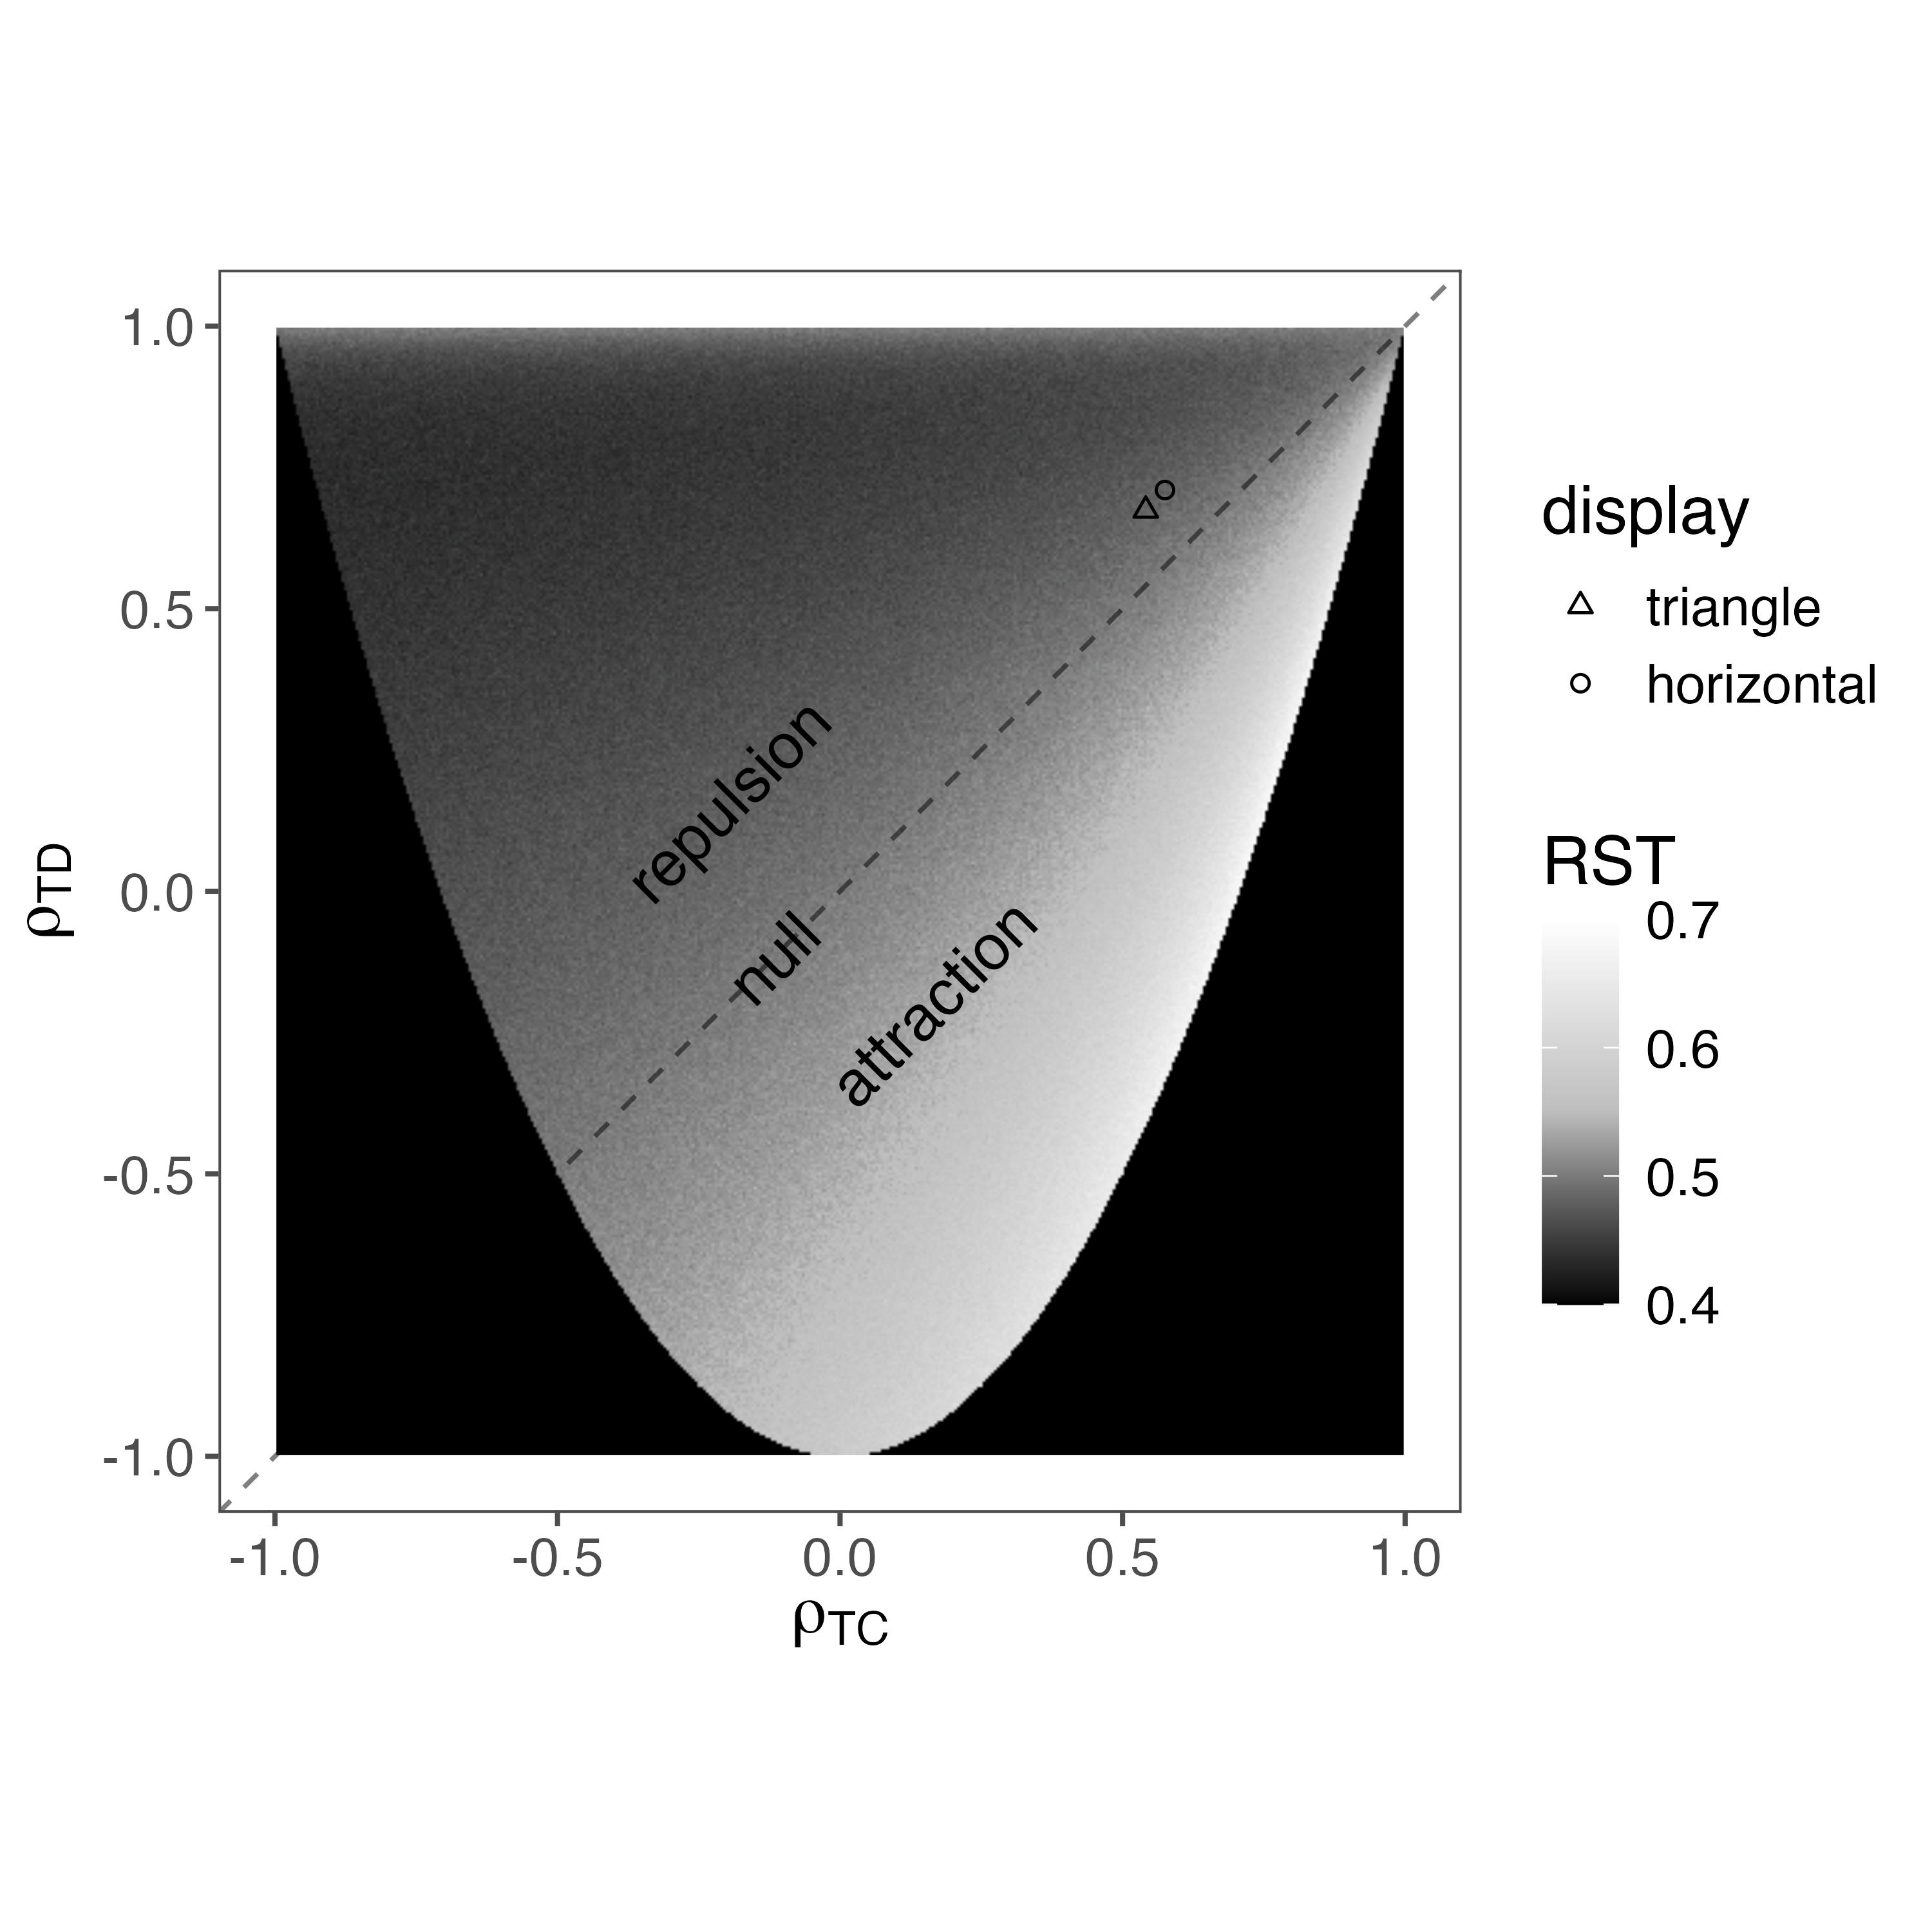
\includegraphics[width=\linewidth]{figures/3d_sim_rst.jpg}
   \caption{Model simulations for the attraction and repulsion effects based on the variation of $\rho_{TD}$ and $\rho_{TC}$. "Regions" of the plot are labeled based on their qualitative predictions for attraction, null, and repulsion effects. The black region is the area where, due to extreme correlations, a positive semi-definite variance-covariance matrix could not be formed and predictions are unavailable. The triangle and circle mark the estimated mean correlations from the Experiment 2 triangle and horizontal conditions, respectively (see below for details).}
   \label{fig:3d_model}
\end{figure}

Lastly If $\rho_{TC}>\rho_{TD}$, the model predicts an attraction effect. The logic here is the similar to the above logic; the decoy and competitor tend to move together, and the decoy is more likely to exceed the competitor than the target. 

\subsection{Perceptual Correlations as Mechanism for the Repulsion Effect}
These perceptual correlations, which cause the decoy to occasionally exceed the target in perceived area, may be, at least partially, driving the repulsion effect in \textcite{spektorWhenGoodLooks2018b}'s data. 

Experiment 1 demonstrated that participants do not always discriminate between the target and decoy (or indeed, competitor and decoy). Experiment 1 also demonstrated the triangle display decreases discriminability relative to the horizontal display.

The target and decoy, however, are quite perceptually similar and easier to compare. Simultaneously, however, the fact that target and decoy share an orientation (i.e., both wide or both tall) makes the comparison of these two options easier. At lower levels of TDD, when discriminability is quite difficult (i.e., the difference between $\mu_{D}$ and $\mu_{T}$/$\mu_{C}$ is small), the similarity of target and decoy makes it more likely the decoy is occasionally perceived as larger than the target, than the competitor. I

In statistical terms, the perception of the decoy is more strongly correlated with the perception of the target than with perception of the competitor. These correlations are measured with the $\rho_{TD}$ and $\rho_{CD}$ parameters. According to this account, if $\rho_{TD}>\rho_{CD}$, the perceived areas of target and decoy "move" together, allowing the competitor to exceed the target at a higher rate than the target exceeds the competitor, particularly if perceptual discriminability is low. This account explains the repulsion effect as a perceptual phenomenon rather than a decision-making phenomenon.

Experiment 2, shown below, combined a psychophysics task with a choice task to estimate the parameters of the Thurstonian perceptual model outlined in the beginning of this chapter. In the first phase of the experiment, participants estimated the size of target, decoy, and competitor rectangles on each trial. The second phase of the experiment was a standard choice exxperiment, replicating \textcite{spektorWhenGoodLooks2018b}'s results. The data from the first phase of Experiment 2 were used to obtain stable estimates of  $\boldsymbol{\mu}$ and $\boldsymbol{\Sigma}$ for the Thurstonian perceptual model. Finally, the model, conditioned on these parameter estimates, naturally predicts a repulsion effect but not an attraction effect.  

\section{Experiment 2}
The goal of this experiment was to estimate the parameters of the model presented above and to clarify the role of perception and decision in producing the repulsion and attraction effects. The Thurstonian model introduced above can predict the repulsion effect and the attraction effect through the perceptual correlation parameters. However, this model can produce many different data patterns (as shown in Figure~\ref{fig:3d_model}), some of which may be consistent with existing choice data but many others which are not. Thus this experiment allows us to estimate the model parameters using a non-decision task.

Furthermore, participants also separately completed a choice task, replicating \textcite{spektorWhenGoodLooks2018b}. This allows us to estimate the parameters of the model using the judgment task and then test the model's ability to predict the results of the choice task. 

Experiment 2 utilized the \textit{method of cross-modal matching} \parencite{stevensCrossmodalityMatchingBrightness1965}, where participants estimate the intensity of a stimulus presented in one modality using a different response modality (e.g., estimating the loudness of a tone by adjusting the brightness of a light). Participants adjusted the size of a circle to match the perceived area for each rectangle. 

The experiment  \textcite{spektorWhenGoodLooks2018b}'s choice data in the second phase of the experiment. In both phases, there was between-participants manipulation to display the rectangle stimuli in either the horizontal or triangle displays of \textcite{spektorWhenGoodLooks2018b}.

\subsection{Methods}
\subsubsection{Participants.}
Data collection took place at the University of Massachusetts Amherst. 521 undergraduate students participated in exchange for course credit. 68 participants did not complete the full experiment within the 1 hour time limit and were removed from all analyses. 10 additional participants were failing at least $2/8$ catch trials from the circle adjustment phase (see below). 

After removing participants, this left $218$ participants in the horizonal display condition and $225$ participants in the triangle display condition. 

Choice trials with RTs $<100\text{ms}$ or $>10,000\text{ms}$ were removed from analysis.

\subsubsection{Stimuli.}
Stimuli were gray-scale rectangles, based on the experiments of \textcite{spektorWhenGoodLooks2018b} and \textcite{trueblood2013not}. 

Both the circle adjustment phase and the choice phase (see below) had critical trials, the main focus of the experiment. On each critical trial, there was a target, competitor, and decoy rectangle. The target and competitor rectangles were always oriented differently (i.e., one wider than tall and the other taller than wide), while the decoy was oriented the same as the target. Target-decoy distance (TDD) also varied, with the decoy being either $2\%$, $5\%$, $9\%$, and $14\%$ smaller than the target and competitor. For example, if TDD=$2\%$, then the decoy's area is $\approx98\%$ the area of the target and competitor. Decoys were created by reducing both the height and width. For example, on the lowest diagonal (see below), the target and competitor had dimension values of $60$ and $135$ px, and the TDD=$2\%$ decoy had dimension values of $59$ and $134$ px. Decoys where both dimension values are lower than that of the target are known as range-frequency decoys in the context effects literature \parencite{wedellDistinguishingModelsContextuallya}. 

To introduce variation in the stimuli, the absolute area of the target and competitor also varied. The target and competitor were either $8100$, $14850$, or $23400$ $\text{px}^2$ (with the decoy area changing proportionally based on TDD), falling along one of three diagonals when plotted. See Figure~\ref{fig:e2_stim} for a plot of all critical stimuli. In pixels, the smaller/larger dimension values on the lower, middle, and upper diagonals were $60/135$, $90/165$, and $120/195$, respectively.
 
\begin{figure}
   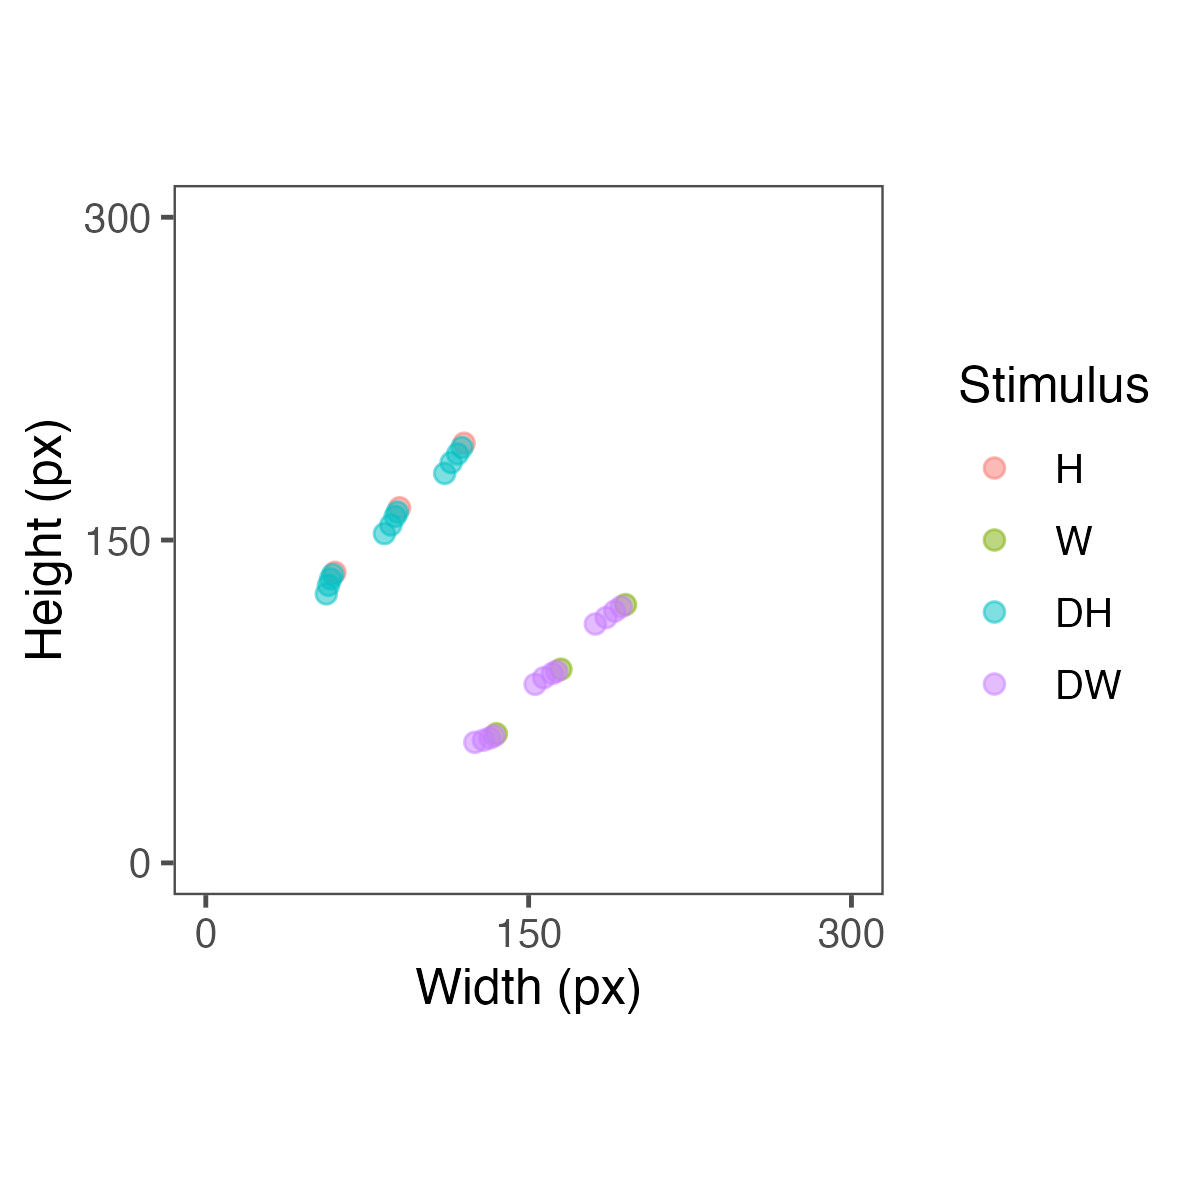
\includegraphics[width=\linewidth]{figures/circle_exp_stim_plot.jpeg}
   \caption{Stimulus configuration for Experiment 2.}
   \label{fig:e2_stim}
\end{figure}

Participants were randomly assigned to either the triangle or horizontal display condition, where, on each trial both rectangles and circles were either arranged in a triangle or in a horizontal array.

The experiment also contained filler trials (see below). On filler trials, stimuli were randomly generated by independently sampling three rectangles' dimension values from the distribution $U(56,195)$px, the full range of dimension values from the critical trials, where $56px$ is the smallest decoy dimension value and $195$ is the largest target/competitor dimension value.

On the catch trials, one larger stimulus was generated by sampling uniformly from the upper diagonal line from the critical trials (see Figure~\ref{fig:e2_stim}). Two additional smaller stimuli were generated by sampling uniformly from the lower diagonal line from the critical trials (see Figure~\ref{fig:e2_stim}). This ensured that one rectangle was always larger than the other two rectangles and allowed for the removal of participants who could not complete the task. Specifically, on a given trial, a participant who did not judge the larger rectangle to be greater in area than the other two rectangles was considered to have "failed" this trial. Only participants who passed $6/8$ judgment catch trials were retained in the analysis (see above).

The choice phase had identical stimuli with the exception that there were no catch trials, only critical and filler trials. Additionally, there were no circles in this phase (see below). 

\subsubsection{Design.}
Across both phases, display condition (triangle, horizontal) varied between-participants and TDD ($2\%$, $5\%$, $9\%$, $14\%$), diagonal (lower, middle, upper), and target-decoy orientation (wide, tall) varied within-participants. 

In the circle adjustment phase, there were 4 blocks, each with 40 trials. Each block consisted of 24 critical trials, 14 filler trials, and 2 catch trials. Within the critical trials, there were 6 trials at each level of TDD. In 3 of these 6 trials the target and decoy were oriented wide (choice set $[W,H,D_{W}]$), and in the other 3 target and decoy were oriented tall (choice set $[W,H,D_{H}]$). 

In the choice phase, there were 4 blocks, each with 34 trials. 24 of these trials were critical trials and 10 were filler trials. Of these 24 critical trials, there were 6 trials at each level of TDD. Within each 6, there were 3 trials where target and decoy were oriented wide and 3 were target and decoy were oriented tall. 

\subsubsection{Procedure.}

The experiment was presented on computer monitors with a resolution of 1920 x 1080 pixels and programmed with GNU Octave \parencite{octave} and PsychoPhysics Toolbox \parencite{brainardPsychophysicsToolbox1997}. 

The experiment took place in two phases: a circle adjustment phase, followed by a choice phase: 

On each circle adjustment trial, participants saw three rectangles and three circles, each labeled 1, 2, and 3. The rectangles appeared in the lower left corner of the screen, either in a triangle or horizontal display, depending on the condition to which the participant was assigned. The circles appeared in the upper right of the screen, in the same display as the rectangles (see Figure~\ref{fig:circle_exp_display} for a sample trial). Stimuli were positioned this way to ensure that participants could not easily compare the circles to the rectangles. A small amount of jitter ($U(-15,15)\text{px}^2$) was also added to the vertical position of each rectangle and the corresponding circle. Each circle appeared with an area of $78 \text{px}^2$, the minimum size allowed in the experiment. 

\begin{figure}
   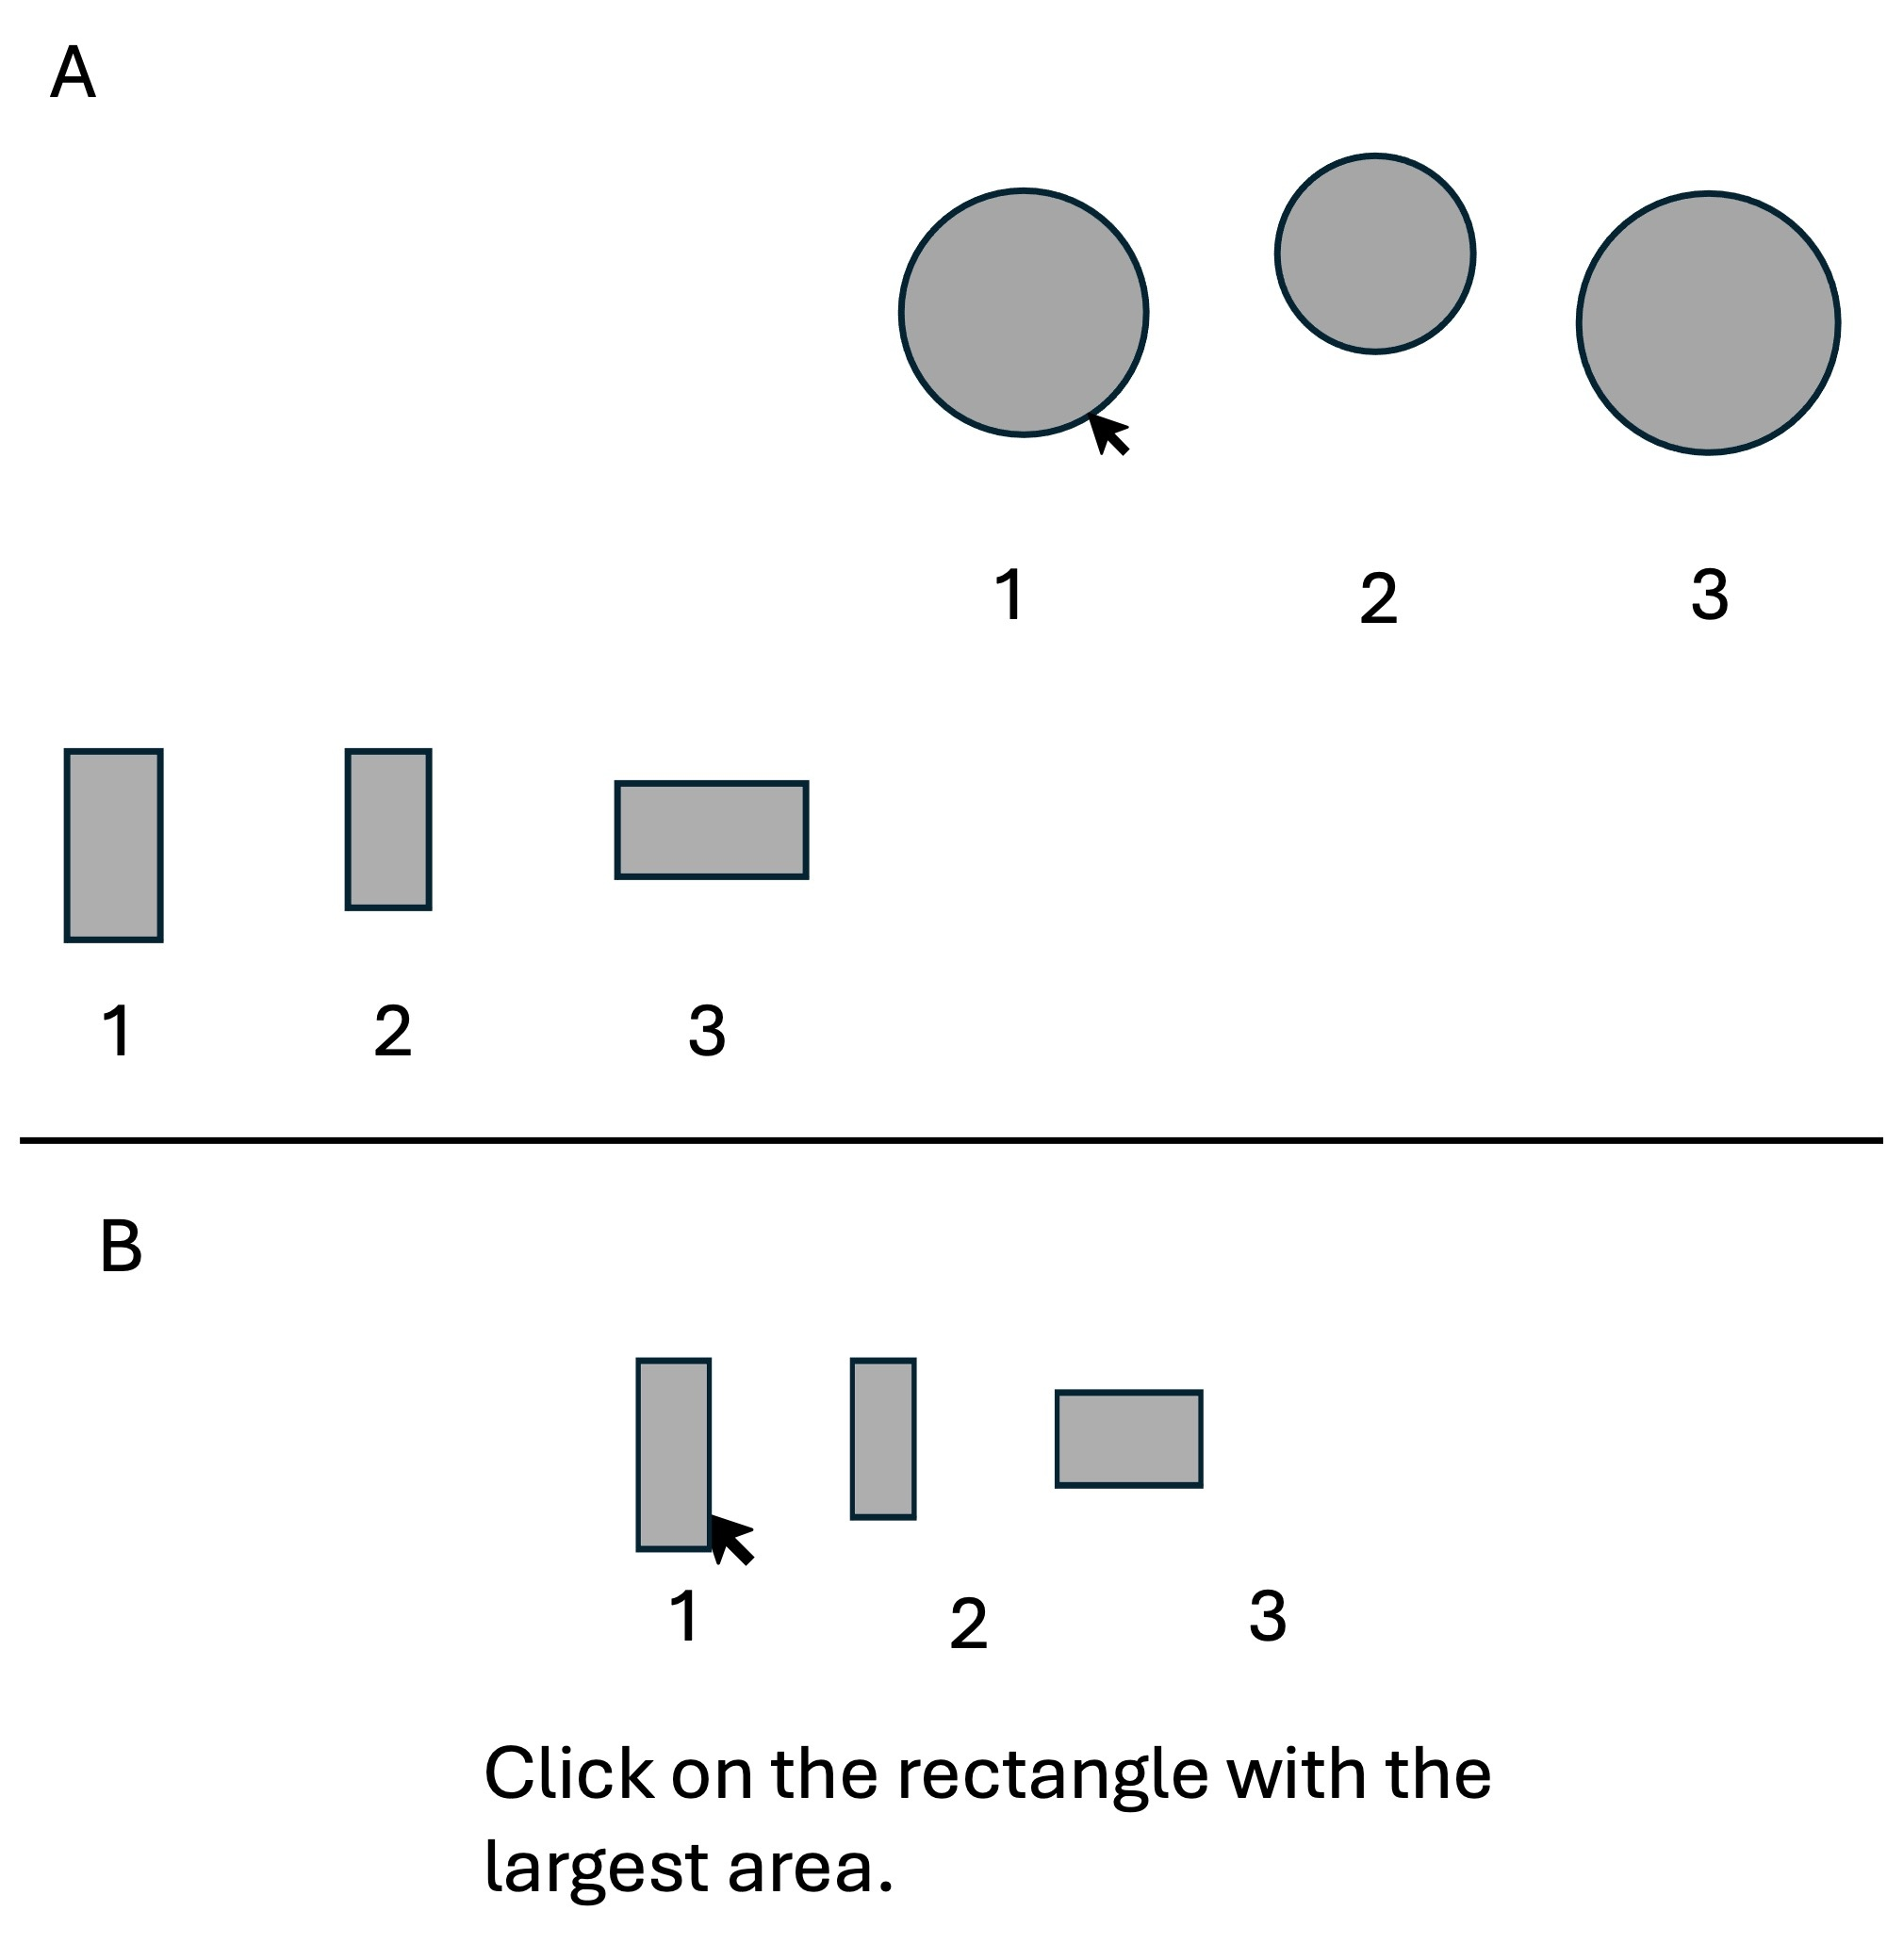
\includegraphics[width=\linewidth]{figures/circle_exp_display.jpg}
   \caption{Example trials from Experiment 2. A: Circle adjustment phase. B: Choice phase. This is an example from the horizontal display condition.}
   \label{fig:circle_exp_display}
\end{figure}

Participants were told to adjust the size of each circle until it had the same area as the rectangle with the corresponding label. They used the mouse to adjust the circles. They were not given instructions on the order they should adjust the circles in or the time they were to spend on the adjustments. The maximum circle area allowed was $65144 \text{px}^2$\footnote{This was the maximum area the circles could be while only appearing on the right half of the screen and maintaining the same horizontal distance from each other as the corresponding rectangles. The minimum possible rectangle area in the experiment was $3136px^2$, while the maximum possible area was $38025px^2$. Thus the range of possible responses was well within the true area of all rectangles.}, and the minimum area was $78 \text{px}^2$. When a participant finished adjusting the circles on a trial, they clicked the "Submit" button located on the lower right hand corner of the screen and advanced to the next trial. 

The circle adjustment phase began with three calibration trials. Calibration trials were identical to filler trials, with the caveat that participants received feedback after their responses. After participants submitted their responses on a calibration trial, a red circle appeared around each adjusted circle, showing the true area of the corresponding rectangle.  

After the calibration trials, the experimental circle adjustment trials began. There were 4 blocks of experimental trials. At the beginning of each block, participants completed $3$ calibration trials. 

At the end of each block, participants were told that they were either over or under-adjusting, on average, based on the current mean deviation of their responses from the true areas. They were not told the magnitude of their over/under-estimation.

After the circle adjustment phase, the choice phase began. During the choice phase, participants were shown three rectangles on each trial and asked to select the rectangle with the largest area. They were told that they would know their percentage of correct choices at the conclusion of the experiment.

The choice phase began with $3$ practice trials, which were identical to the filler trials but separate from the experiment. Participants did not receive feedback during choice practice trials. 

At the end of the choice phase, participants were told their percentage of correct choices. Note that in a critical trial, a correct response is one where the participant did not select the decoy, given that the target and competitor rectangles always had the same area.

In both the circle phase and the choice phase, stimulus order was randomized on each trial.

\subsection{Results}
\subsubsection{Data Processing}

These data required processing to ensure that no outliers influenced estimates of $\boldsymbol{\mu}$ or $\mathbf{\Omega}$, as it is widely known that outliers can detrimentally influence correlation estimates. 

The most substantial data processing occured in the circle phase data, so these are discussed first.

First, all trials where at least one circle was not adjusted (i.e.,
at least one circle was left at the starting size) were removed. Given the discrepancy between the starting circle area ($78\text{px}^2$) and the smallest rectangle area shown in the experiment ($3,136\text{px}^2$), these are unlikely to be representative of any participant's true perception of rectangle area.

Next, outlier participants were removed, followed by outlier trials from the remaining participants. An outlier participant is a participant is one whose responses are substantially different from most other participants, while an outlier trial is a trial, from a valid participant, which differs substantially from the rest of a given participant's trials. Outlier participants were first removed, and then outlier trials were removed from the remaining participants.

Outlier participants were identified and removed using the following procedure:

Each individual participant's data were log-transformed\footnote{This was done to reduce the skewness observed in the raw data.}. Each participant's data were then fit to a linear regression, regressing each log circle area on each corresponding log rectangle area. Participants whose corresponding $R^2$ value fell below the $5\%$ quantile for all $R^2$s ($.3975$ in this case) were removed from all analysis. The $5\%$ quantile was chosen arbitrarily as a conservative threshold to ensure maximum participant retention while removing outliers. 

This procedure removed $23$ participants, leaving $N=420$ participants, $213$ in the triangle display condition and $207$ in the horizontal display condition. Of the remaining participants, $R^2$ values were high ($M=.67,SD=.12$), indicating that participants could generally perform the task.

Next, outlier trials were identified and removed using the following procedure:

From the $420$ partipants whose data were analyzed, outlier trials were removed from the critical trial data. All data points were then z-transformed within each participant and diagonal\footnote{This was done solely for the removal of outliers, not for the substantive analysis that followed.}. All critical trials with at least one z-score with an absolute value above $3.5$ were dropped, removing a total of $102$ trials. This removed $0$, $1$, $2$, and $4$ critical trials from $339$, $62$, $18$, and $1$ participants, respectively. This left $20371$ data points in the triangle display condition and $19809$ data points in the horizontal display condition, where a data point is a vector of the participant's estimated target, competitor, and decoy areas on a given trial. 

Only those participants whose data were retained in the circle adjustment phase were retained in the choice phase. 

\subsubsection{Circle Adjustment Phase Results}

First, it is important to show that participants could adequately perform the adjustment task. The mean difference between actual log area and estimated log area was computed for each participant, stimulus pair (i.e., target-competitor, target-decoy, competitor-decoy), and actual difference. These results are plotted in Figure~\ref{fig:circle_boxplots}. The x axis shows the actual difference between areas, while the y axis shows the estimated difference in areas according to participants' judgments. Participants' judgments varied considerably along the y axis, but on average, the estimated difference increased with the actual difference. 

\begin{figure}
   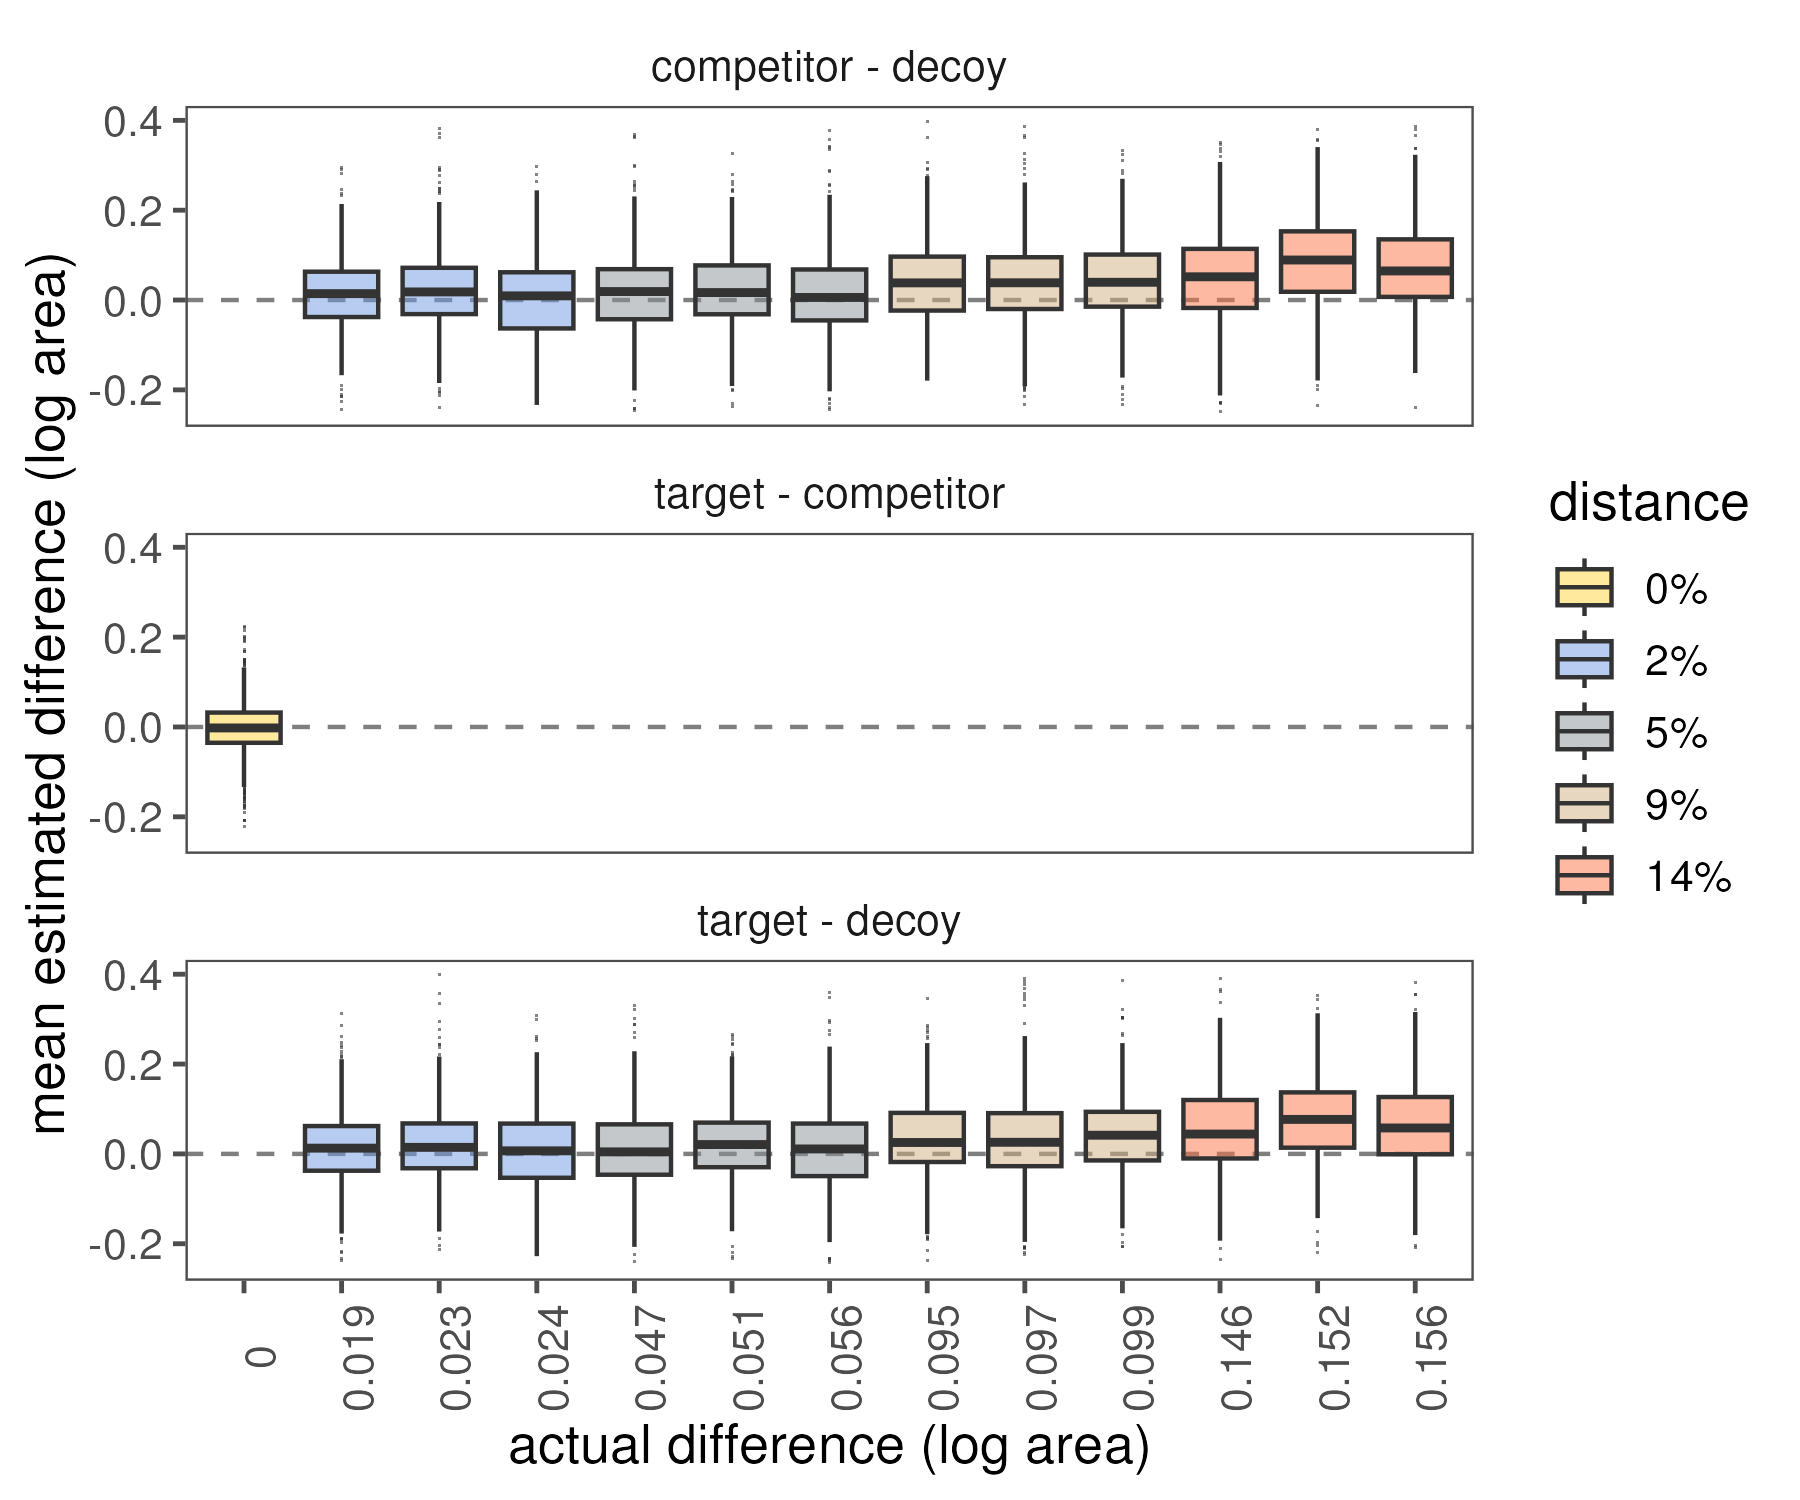
\includegraphics[width=\textwidth]{figures/circleAreaPhase_boxplot_meanlogdiffs_no_outliers.jpeg}
   \caption{Experiment 2 plots of subject-level mean error in log-transformed area estimations, split by stimulus pair (e.g., target-decoy), TDD, and actual difference in rectangle area. Because the difference in physical area at a given TDD differed across the three diagonals, there are three plots per each TDD level. Note that because the target and competitor rectangles always had equal areas, the true difference is always 0.}
   \label{fig:circle_boxplots}
\end{figure}

Next scatterplots of all pairwise circle area estimations are shown in Figure~\ref{fig:raw_cors}. 

Correlation coefficients in each display condition were also computed. For the triangle condition, $r_{td}=.61$, $r_{cd}=.54$, and $r_{tc}=.55$. For the horizontal condition, $r_{td}=.66$, $r_{cd}=.56$, and $r_{tc}=.57$. In both conditions, the target-decoy correlation is stronger than both the competitor-decoy and the target-decoy correlations. 

\begin{figure}
   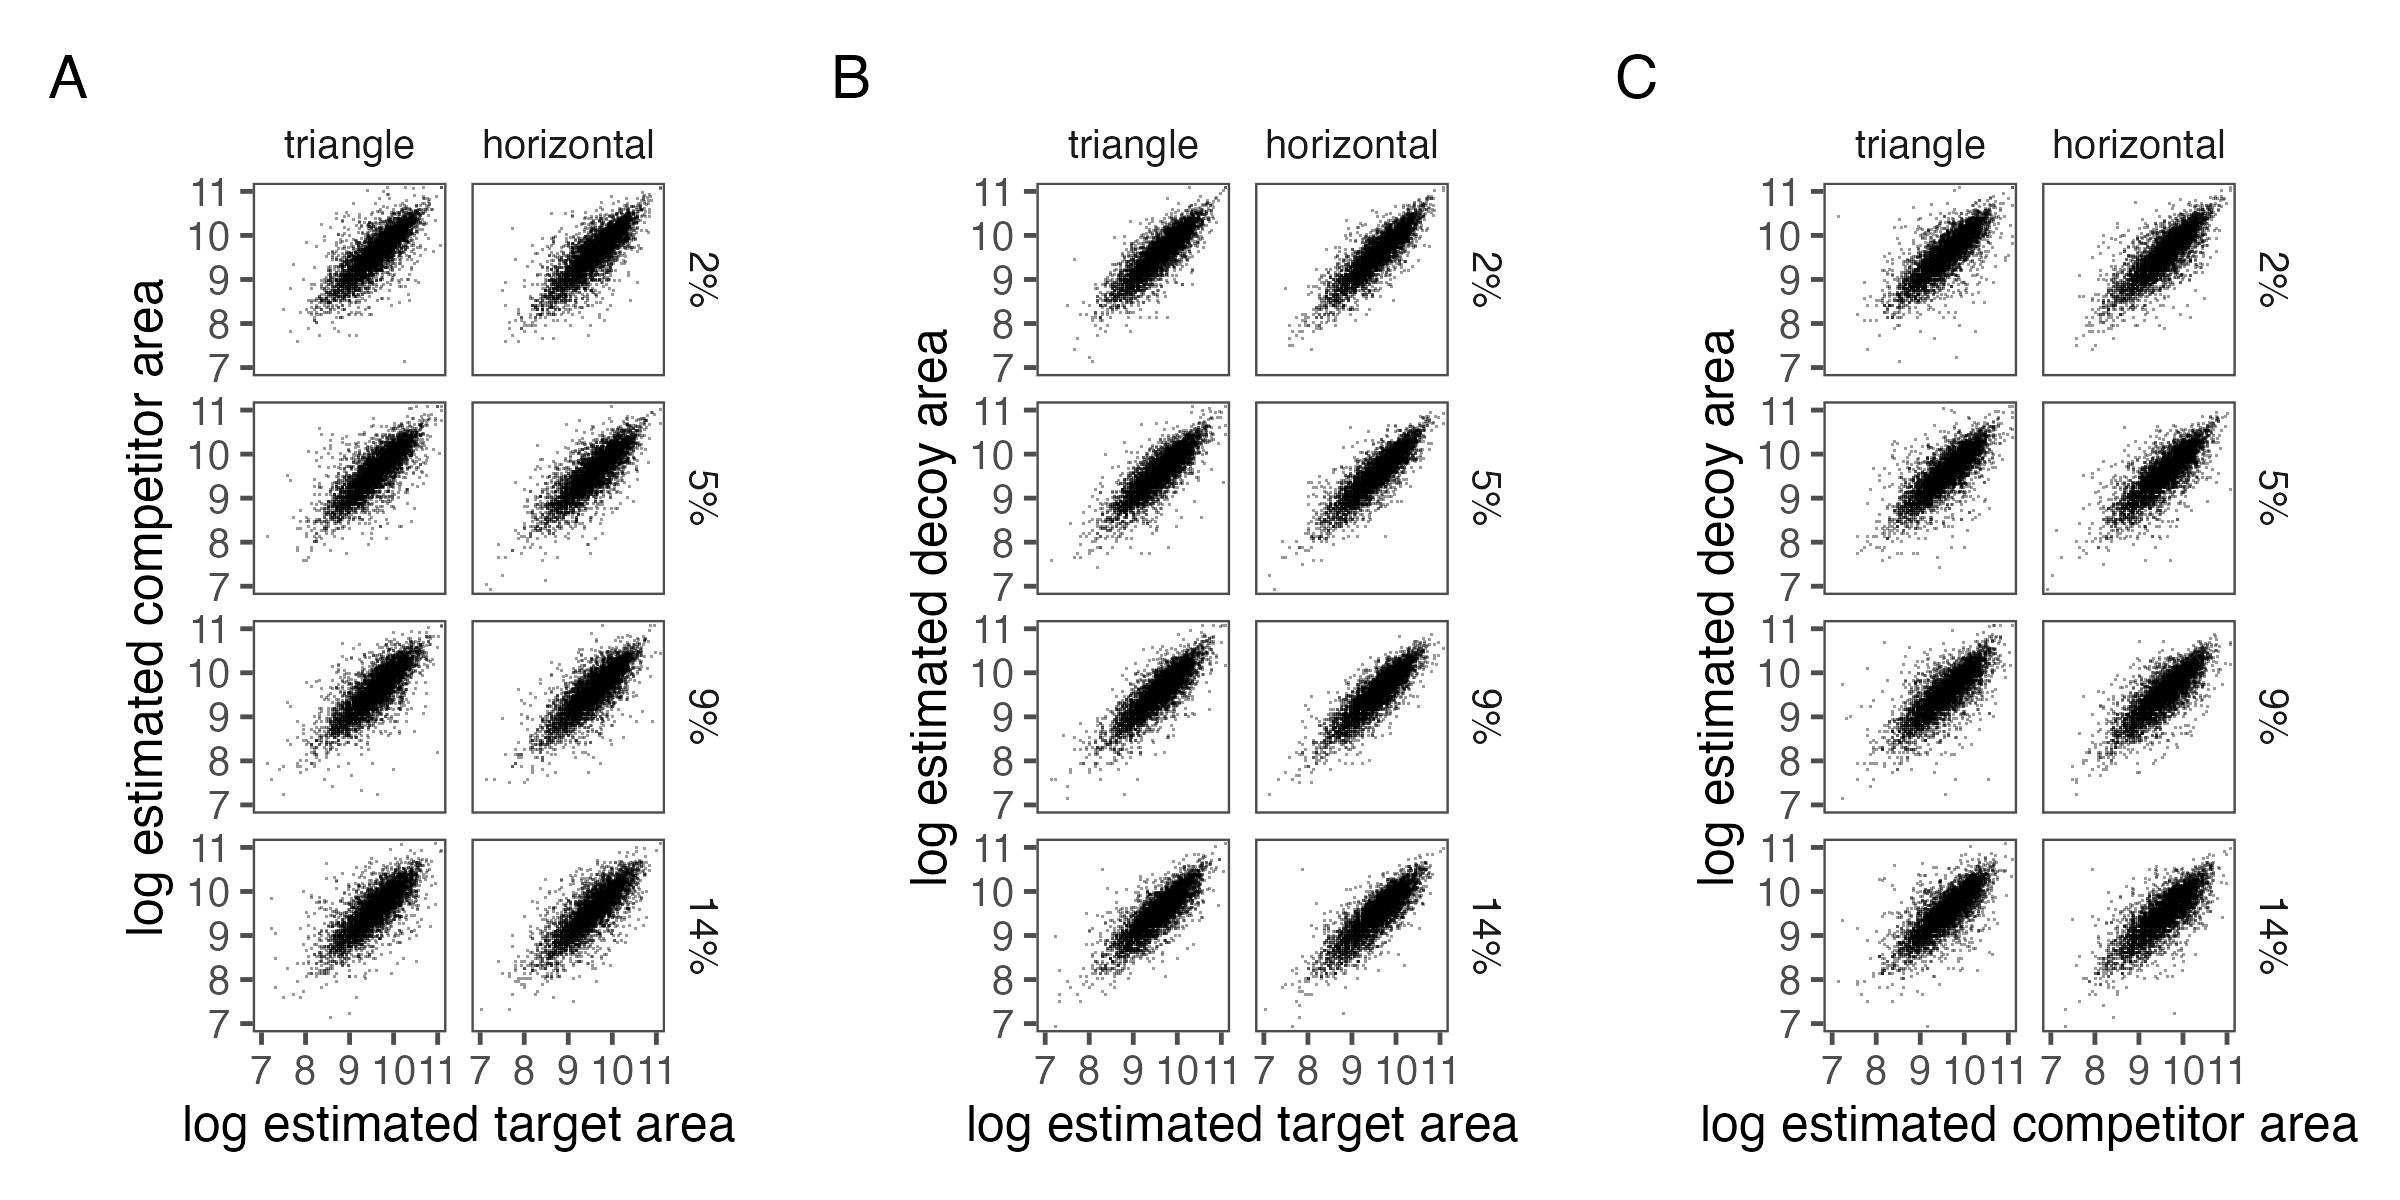
\includegraphics[width=\textwidth]{figures/circleAreaPhase_cor_plot_all_no_outliers.jpg}
   \caption{Scatterplots of target-decoy (left), competitor-decoy (middle), and target-competitor (right) log estimated areas, split by display condition (columns) and TDD (rows).}
   \label{fig:raw_cors}
\end{figure}

Bayesian hierarchical modeling was used to estimate the parameters of the Thurstonian perceptual model introduced earlier, as well as perform inference on the means and correlations. Though the descriptive parameter estimates are also reported, the Bayesian analysis allows estimating the posterior distributions on each relevant parameter and comparing the range of plausible values across parameters and conditions. Furthermore, the Bayesian hierarchical modeling also takes into account participant-level differences in area estimation. 

As an alternative to computing descriptive statistics for the relevant components of a multivariate Gaussian (i.e., computing raw means, variances, and correlations), the Bayesian analysis allows us to model the obtained trial-level area judgments as coming from a single joint Gaussian distribution of estimated areas. Additionally, this is also a novel application of the multinomial probit (MNP) model, whose parameters are usually estimated by inferring utilities from choice data \parencite{train2009discrete}. In the current application, the parameters are estimated from the judgment data using Bayesian modeling and used to predict choice data, which were collected from the same participants. 

The main text contains estimates of $\boldsymbol{\mu}$ and $\boldsymbol{\Sigma}$ (the vector of means and the variance-covariance, respectively), while the details of the estimation procedure are found in the Appendix. As discussed above $\boldsymbol{\Sigma}$ is a positive semi-definite variance-covariance matrix, computed as $\boldsymbol{\Sigma}=S\boldsymbol{\Omega}S$, where $S$ is a vector of standard deviations and $\boldsymbol{\Omega}$ is a $3\text{x}3$ correlation matrix. 

The estimates of $S$ suggest no systematic differences in the variance of area judgments variance across target, decoy, and competitor rectangles. In the triangle condition, the parameters were as follows: $\sigma_{T}$:\textit{M}$=0.34$,\textit{SD}$=0.002$,$95\%\text{HDI}$ $[0.332,0.338]$, $\sigma_{C}$:\textit{M}$=0.34$,\textit{SD}$=0.002$,$95\%\text{HDI}$ $[0.335,0.341]$, $\sigma_{D}$:\textit{M}$=0.34$,\textit{SD}$=0.002$,$95\%\text{HDI}$ $[0.331,0.338]$. In the horizontal condition, the parameters were as follows: $\sigma_{T}$:\textit{M}$=0.34$,\textit{SD}$=0.002$,$95\%\text{HDI}$ $[0.334,0.340]$, $\sigma_{C}$:\textit{M}$=0.34$,\textit{SD}$=0.002$,$95\%\text{HDI}$ $[0.338,0.345]$, $\sigma_{D}$:\textit{M}$=0.34$,\textit{SD}$=0.002$,$95\%\text{HDI}$ $[0.333,0.340]$. 

Estimates of the $\boldsymbol{\mu}$ components at each TDD level (averaged across participants) are plotted in Figure~\ref{fig:e2mu}. First, note that the decoy mean is always lower than that of the target and competitor. Furthermore, as TDD increases, the decoy mean decreases, indicating that participants were sensitive to decreases in absolute area, judging smaller rectangles as having smaller areas. Both target and competitor mean areas also decrease with TDD, suggesting that participants somewhat adjusted these areas relative to the decoy. 

Focusing solely on the target and competitor means, an interesting pattern emerges. The competitor mean is always larger than the target mean, albeit only slightly (see Appendix for details). This pattern is somewhat consistent with the tainting hypothesis, the idea that nearby decoys can taint the value of target option \parencite{simonson2014vices}. However, the tainting hypothesis predicts that tainting is a decreasing function of distance in attribute space, and the current observed difference between target and competitor means appears to be constant. There is also limited statistical evidence for this difference, as the $95\%$ HDIs overlap considerably at each TDD level in both display conditions (see Figure~\ref{fig:e2mu}). 

There is, however, evidence from the Bayesian Hierarchical Regression (see Appendix), via the competitor-specific regression coefficient $\beta_{comp}$, that the competitor is rated higher than the target, at least in the triangle condition. The $\beta_{comp}$ parameter captures the tendency for participants to rate the competitor higher than the target, regardless of the TDD or target orientation. In the triangle condition, this parameter was reliably above 0, \textit{M}$=0.005$, \textit{SD}$=0.0023$, $95\%\text{HDI}$ $[0.0001,0.009]$. Note that this effect is quite small. Given that the data were transformed via the natural logarithm, this estimate corresponds to a $e^{0.005}=1.005\text{px}^2$ difference in mean judged area, a considerably small effect size. In the horizontal condition, this parameter was not reliably different from zero, \textit{M}$=0.003$, \textit{SD}$=0.002$, $95\%\text{HDI}$ $[-0.002,0.007]$. 

The estimates of $\boldsymbol{\Omega}$ (the correlations) are plotted in Figure~\ref{fig:e2_omega}. First, it is worth noting that all correlations are positive. This means that in general, there are strong trial-level dependencies between area judgments. However, the crucial pattern emerges when comparing the correlations to one another within each display condition. As predicted, in both display conditions, $\rho_{TD}$ is larger than both $\rho_{CD}$ and $\rho_{TC}$, while $\rho_{CD}$ and $\rho_{TC}$ do not differ from each other. This shows that there is a stronger dependency between judgments of the target and decoy (which are perceptually similar to one another) than of the target and competitor or the competitor and decoy.  

The relatively high $\rho_{TD}$ estimate predicts that the target and decoy tend to "move" together. On trials where the target is judged relatively large, the decoy is also judged to be relatively large. Furthermore, because $\rho_{TD}>\rho_{CD}$, this means that the decoy is more likely to be judged larger than the target than it is to be judged larger than the competitor. This provides a plausible mechanism for the repulsion effect; the decoy is more likely to steal choice shares away from the target than from the competitor. This can generate a data pattern where $P(C)>P(T)$ without requiring $\mu_{C}>\mu_{T}$. 

Furthermore, all $\rho$ parameters from the horizontal condition are larger than the corresponding parameters from the triangle condition. This suggests that the difference between area judgments for target, competitor, and decoy rectangles in the horizontal condition can be more attributed to the true differences between their means than to general noise, when compared to the triangle condition. However, given that the model was fit separately to each display condition, these inferences should be considered cautiously.

\begin{figure}
   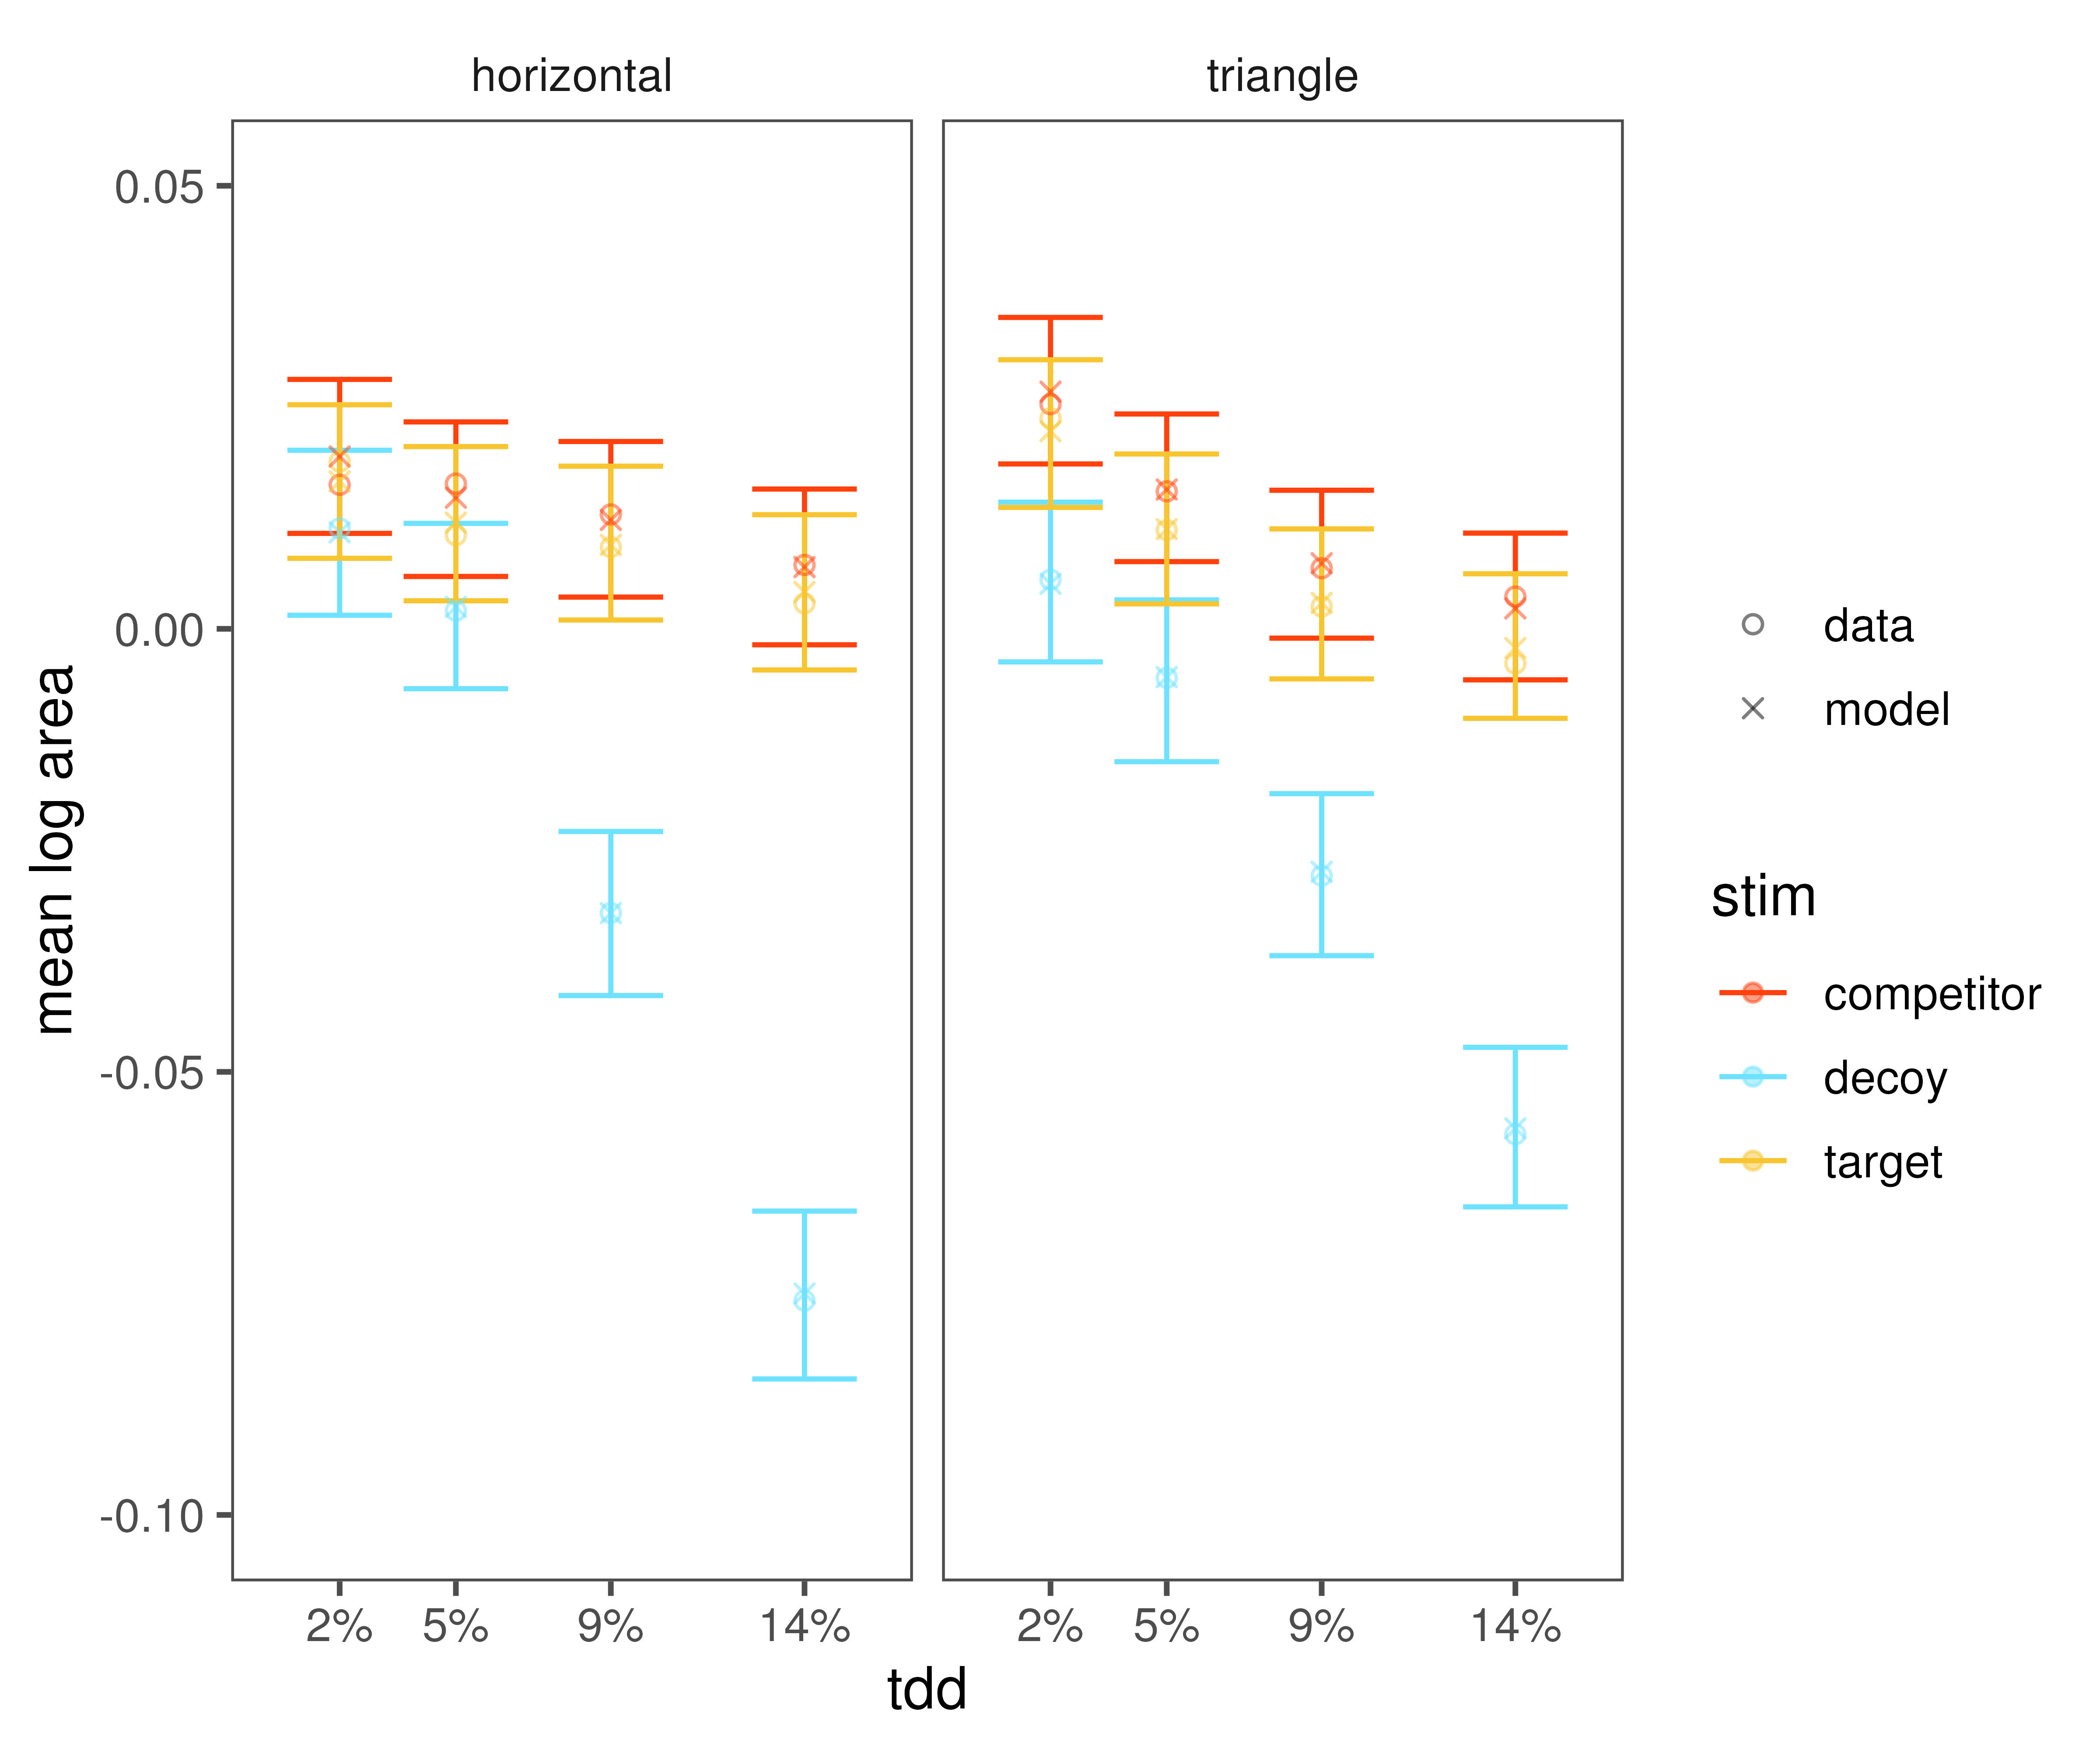
\includegraphics[width=100mm]{figures/bayes_circle_area_mu_sigma_constant_comp_effect_model_v_data_collapsed.jpeg}
   \caption{Experiment 2 $\boldsymbol{\mu}$ estimates. Model values are means, and the error bars are $95\%$ HDIs.}
   \label{fig:e2mu}
\end{figure}

\begin{figure}
   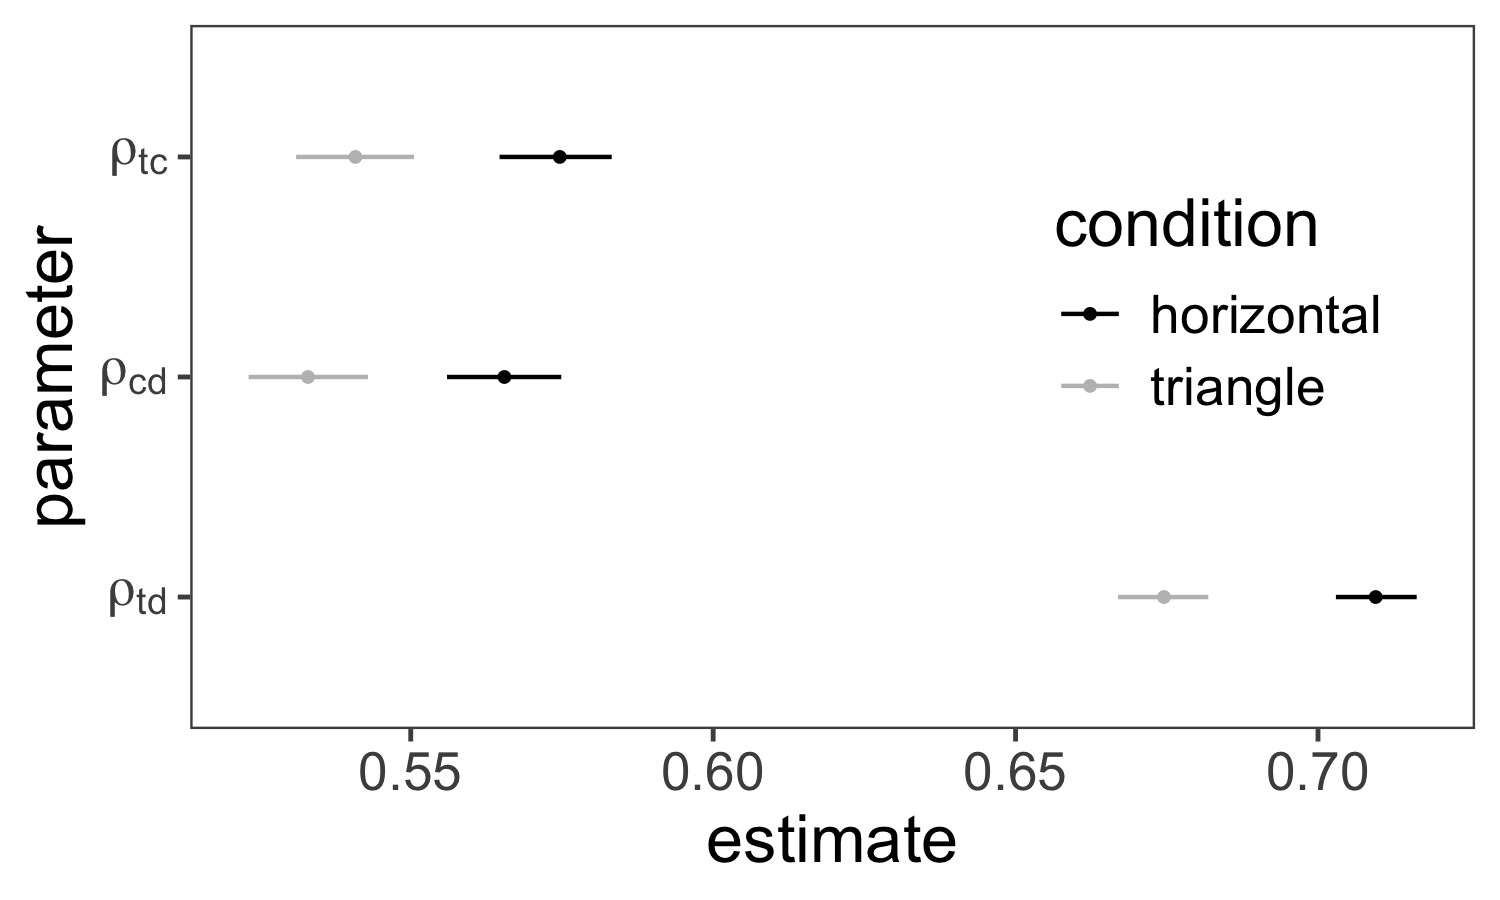
\includegraphics[width=100mm]{figures/bayes_circle_area_sigma_constant_comp_effect_omega_plot.jpeg}
   \caption{Experiment 2 posterior estimates of $\boldsymbol{\Omega}$ off-diagonal parameters across display conditions. Lines show $95\%$ HDIs. Dots indicate means.}
   \label{fig:e2_omega}
\end{figure}

\subsubsection{Choice Phase Results}

In each trial of the choice phase, participants saw three rectangles and selected the rectangle with the largest area. This was a replication of \textcite{spektorWhenGoodLooks2018b}.

Mean choice proportions across display condition and TDD are plotted in Figure~\ref{fig:e2_choiceprops}, collapsed across choice set (i.e., ignoring whether the target was wide/tall). 

First, in both display conditions, note that decoy choice decreases with TDD. Participants were sensitive to the absolute size of the decoy and chose it less often as the decoy decreased in area. 

In the triangle condition (Figure~\ref{fig:e2_choiceprops}, left panel), at the first three levels of TDD (i.e,. $2\%$, $5\%$, and $9\%$), the data show a fairly strong repulsion effect, as the competitor was clearly chosen more often than the target. Though this figure suggests a null effect at $TDD=14\%$, inferential statistics on AST (Absolute Share of the Target) show that there is also a slight repulsion effect at $TDD=14\%$ (see Appendix). 

In the triangle condition (Figure~\ref{fig:e2_choiceprops}, left panel), at the first two levels of TDD (i.e,. $2\%$ and $5\%$), the data show a fairly strong repulsion effect, as the competitor was clearly chosen more often than the target. Though this figure suggests an attraction effect at $TDD=9\%$, inferential statistics on AST (Absolute Share of the Target) show that there is a null effect at $TDD=9\%$ (see Appendix). The data clearly show, however, a strong attraction effect at $TDD=14\%$. See the Appendix for inferential statistics which support these conclusions.

\begin{figure}
   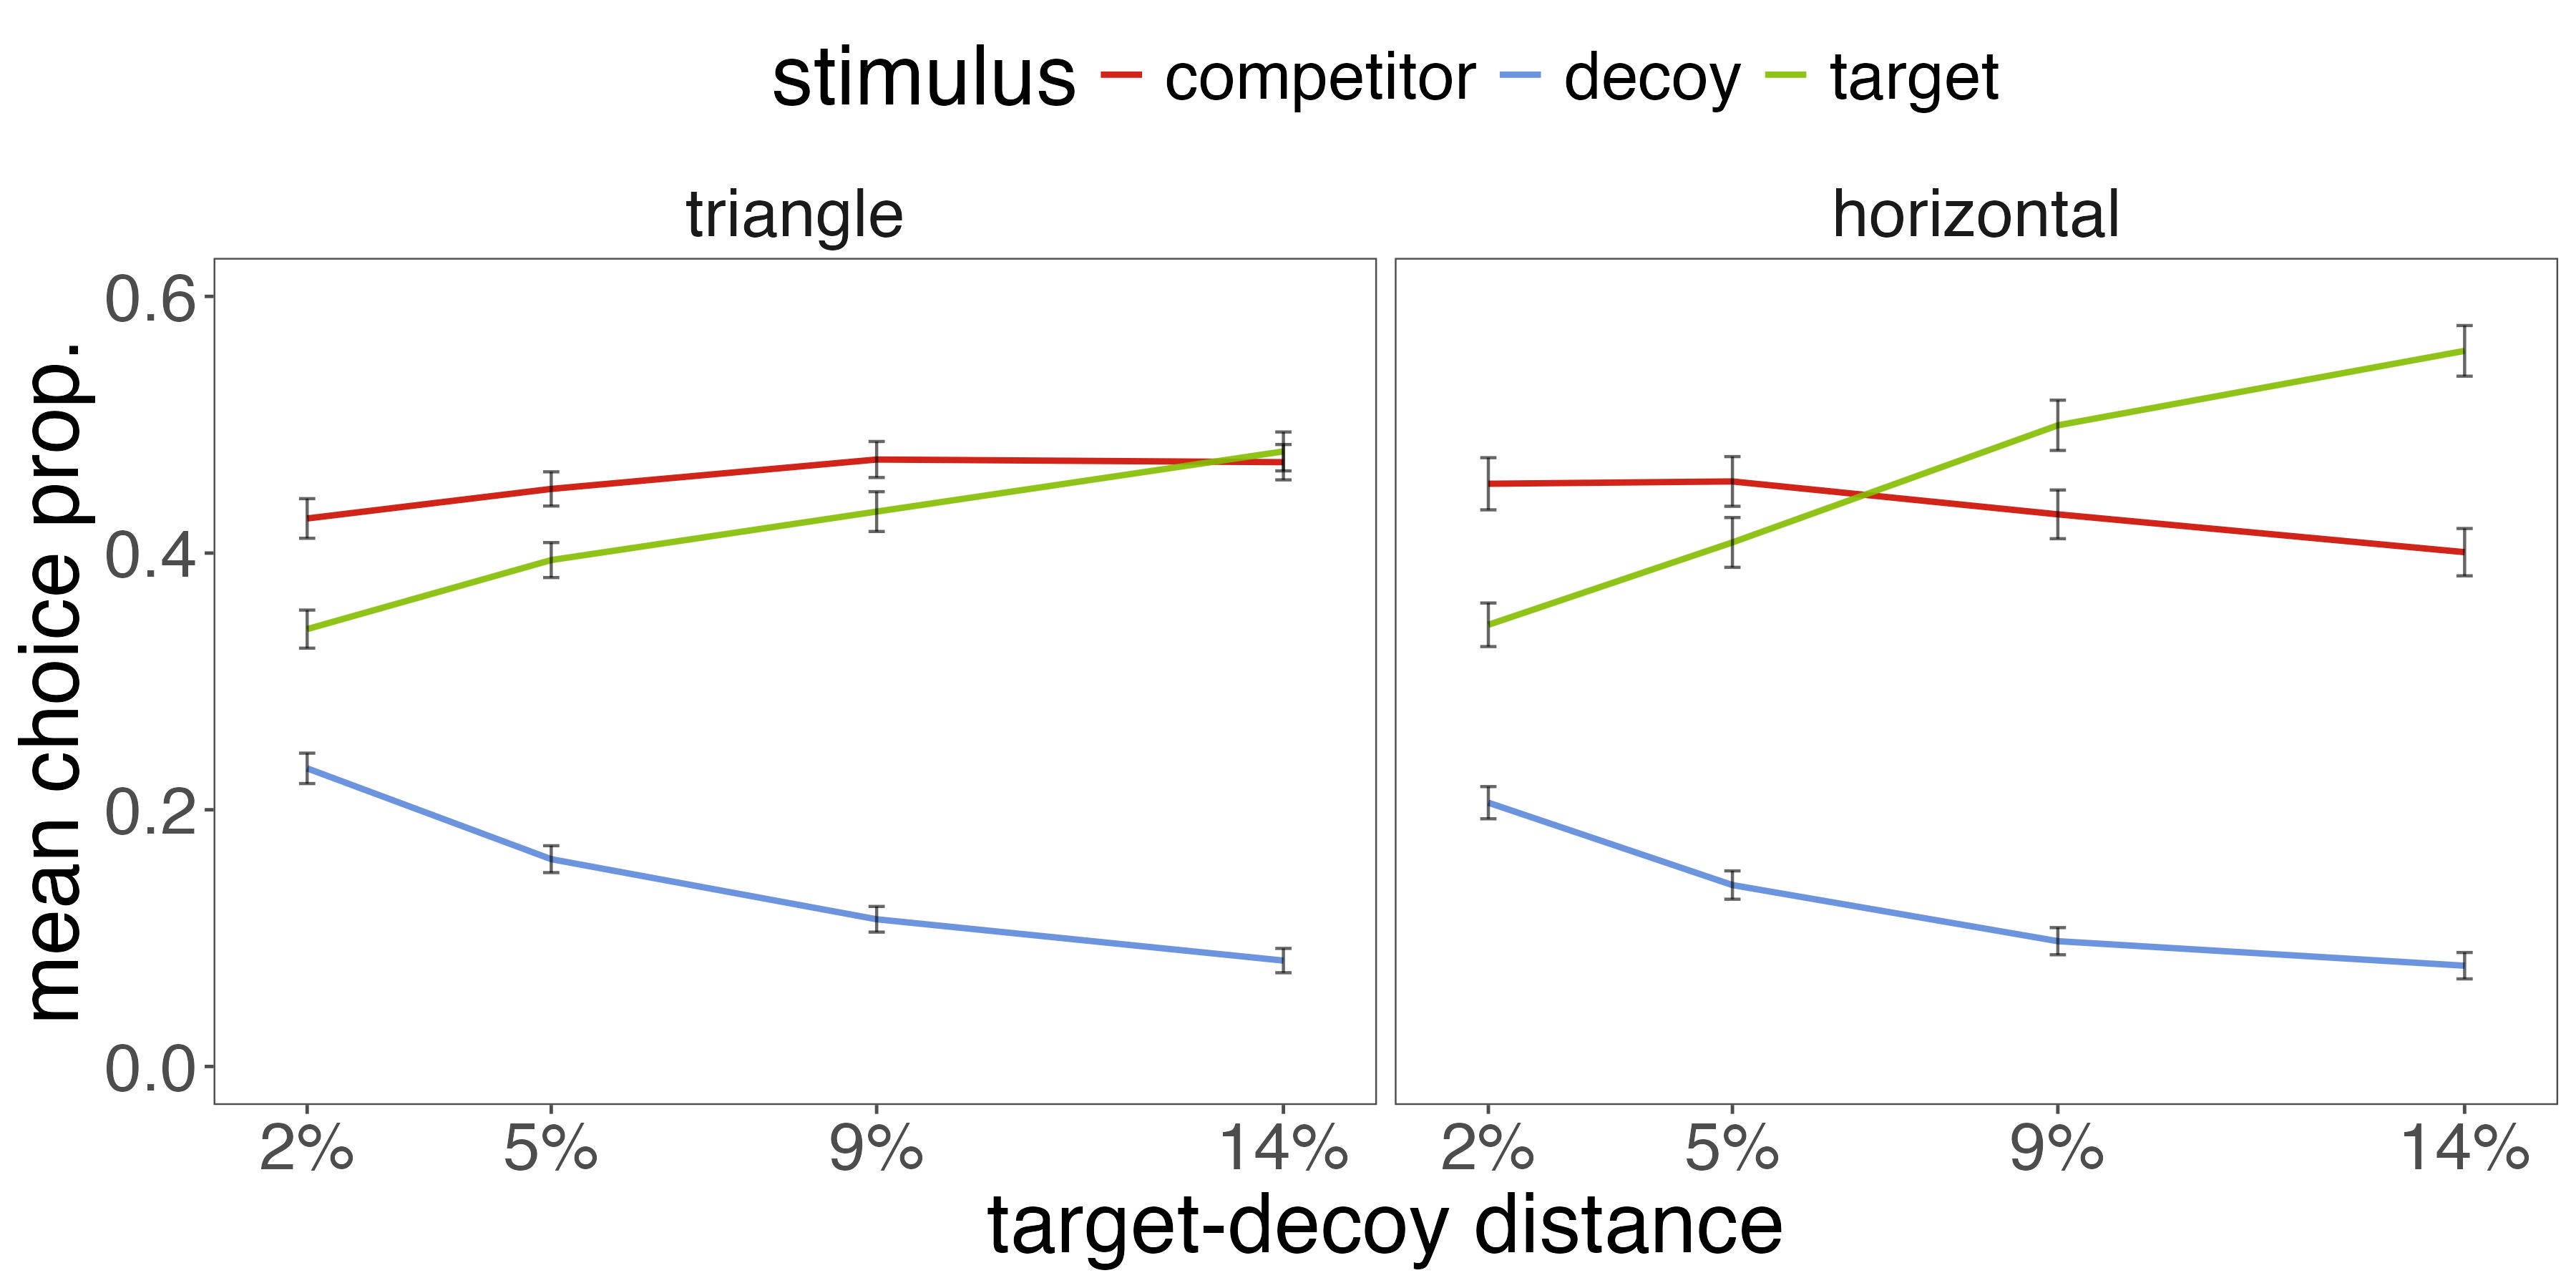
\includegraphics[width=\textwidth]{figures/choicePhase_att_trials_mean_choice_props_collapsed.jpg}
   \caption{Experiment 2 mean choice proportions for target, competitor, and decoy options, by TDD and display condition. Error bars are $95\%$ CIs on the means.}
   \label{fig:e2_choiceprops}
\end{figure}

These data show that the repulsion effect, at least in the current paradigm, is strongly related to the similarity between target and decoy along with participants' ability to discriminate the target/competitor from the decoy. As TDD increases, the repulsion effect either decreases in magnitude (triangle condition) or reverses entirely, to an attraction effect (horizontal condition). The results are also consistent with the overall discriminability difference between display conditions. The results of Experiment 1 showed that participants are better at discriminating the target and competitor in the horizontal condition than in the triangle condition. 

To demonstrate the strong relationship between discriminability and the repulsion/attraction effects, the choice data from Experiment 2 are plotted against the two-alternative forced choice data from Experiment 1 (see Figure~\ref{fig:e2_choice_compare_to_2afc}). The y axis is identical to that of Figure~\ref{fig:e2_choiceprops}. However, rather than the TDD - the physical difference between target and decoy - the x axis is now the mean target-decoy discriminability. In other words, the x axis is now the psychological target-decoy difference as rather than the physical difference. 

When the data are plotted this way, a critical pattern emerges. The crossover point - the point at which the repulsion effect becomes null - occurs at lower discriminability levels in the horizontal condition compared to the triangle condition. This strongly suggests that the target-decoy relationship is crucial for generating the repulsion effect.

\begin{figure}
   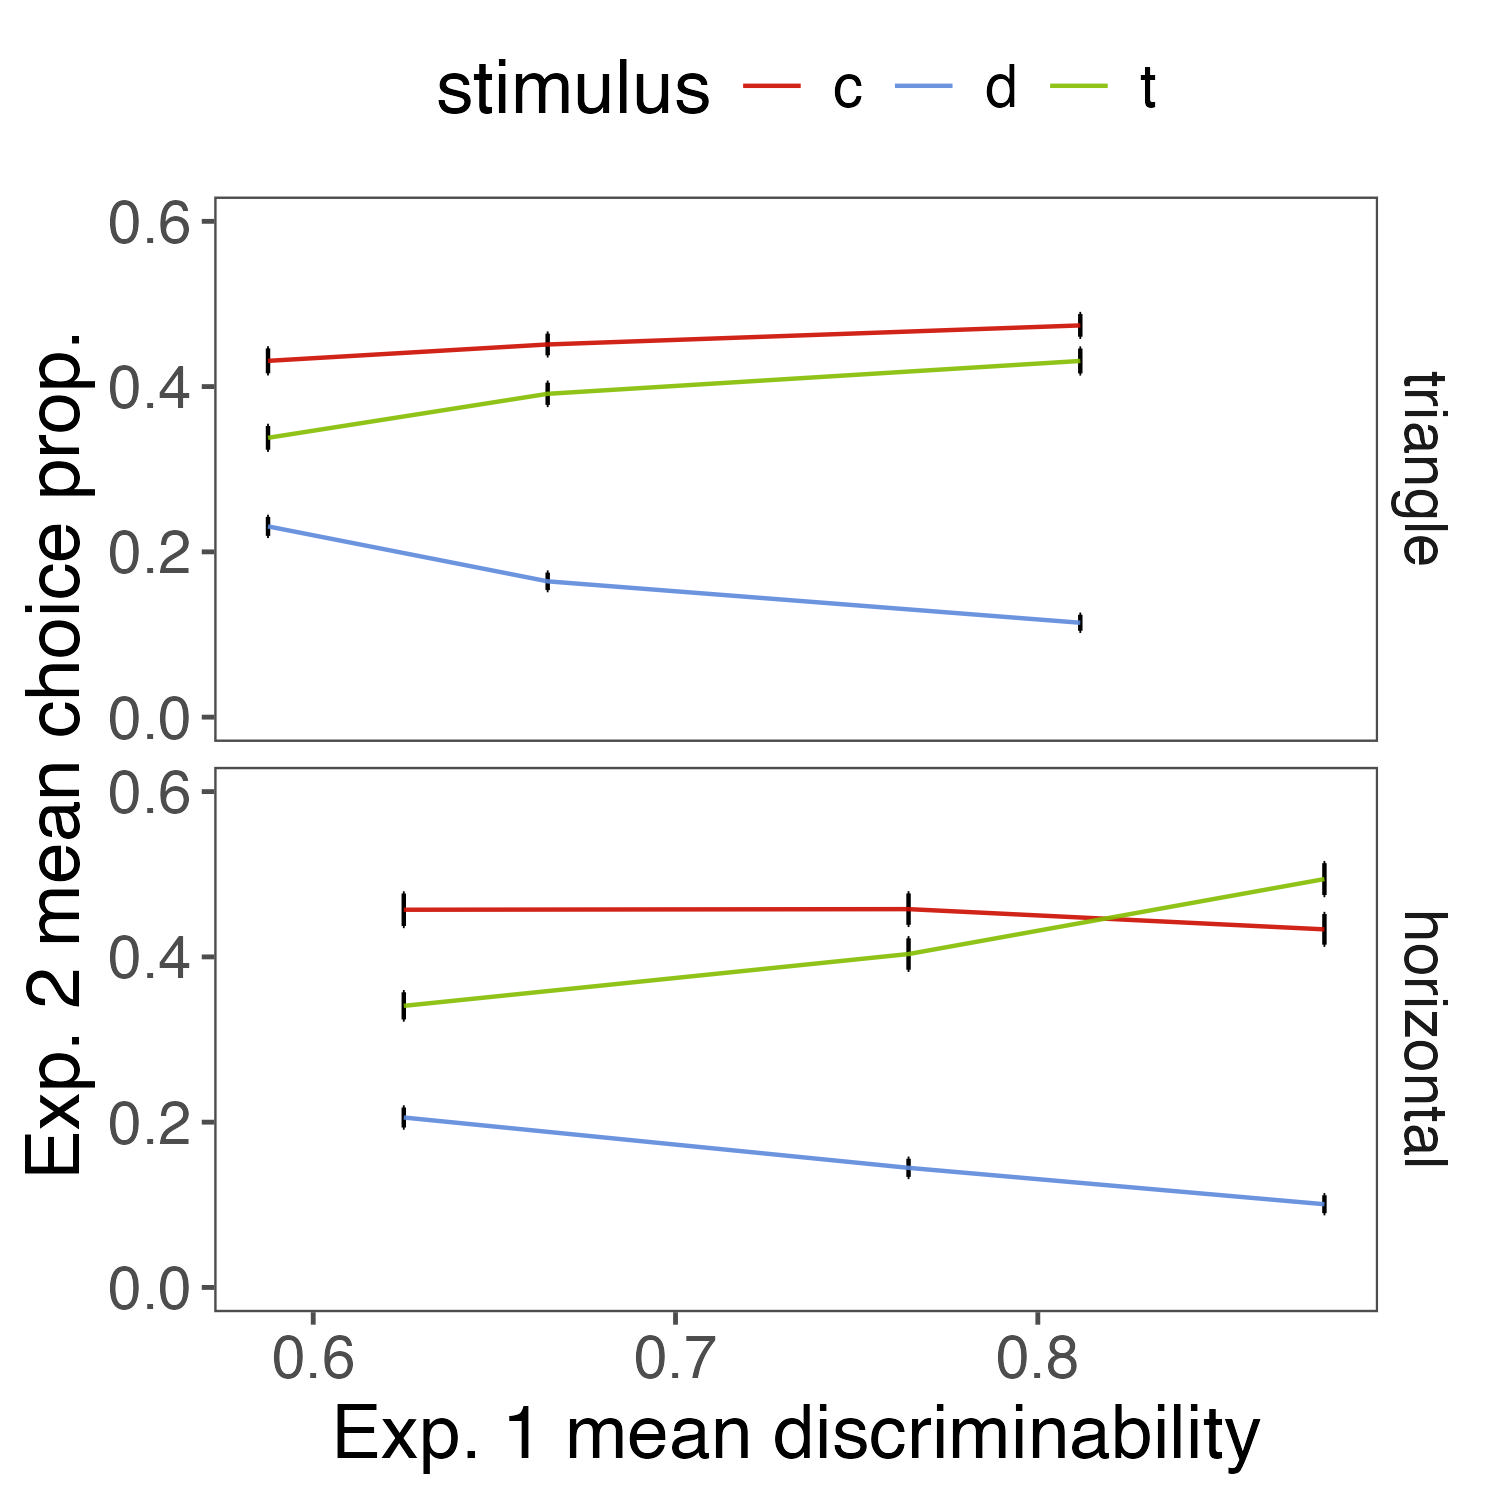
\includegraphics[width=\textwidth]{figures/choicePhase_att_trials_compare_to_2afc_collapsed.jpeg}
   \caption{Mean target, competitor, and decoy choice proportions (y axis) at each TDD level in Experiment 2, plotted against mean target-decoy discriminability for each TDD level from Experiment 1 (x axis). The y axis error bars are $95\%$ CIs on the mean.}
   \label{fig:e2_choice_compare_to_2afc}
\end{figure}

\subsection{Model Simulations}
Earlier in this chapter, it was shown the Thurstonian Choice Model could generate a repulsion effect, an attraction effect, or a null effect, depending on the correlation parameters. However, it was open question whether, conditioned on actual estimated parameters, the model could generate data that match empirical choice data. The goal of the following analysis is to test the model's ability to predict the data. 

Predictions were generated at each level of TDD using the mean estimates of $\boldsymbol{\mu}$\footnote{Given the considerable overlap in HDIs(see Figure~\ref{fig:e2mu}), the $\mu_{T}$ and $\mu_{C}$ parameters were constrained to be equal at each level of TDD. } and $\boldsymbol{\Sigma}$, in each display condition. For simplicity, the mean estimates for each parameter were used, rather than the full distribution of parameter values.

To generate predictions, at each TDD level in each display condition, $1,000,000$ samples were drawn from a multivariate Gaussian distribution with parameters $\boldsymbol{\mu}$ and $\boldsymbol{\Sigma}$, where a sample is a vector of perceived target, competitor, and decoy areas. The choice proportion for each rectangle is simply the proportion of times that a particular rectangle was perceived to be the largest in that sample. The results are plotted in Figure~\ref{fig:e2_model_preds} at each TDD level in each display condition. The reader can also see Figure~\ref{fig:3d_model} to examine where these predictions fall, though Figure~\ref{fig:3d_model} was generated by making assumptions about the mean and variance parameters (see above). 

\begin{figure}
   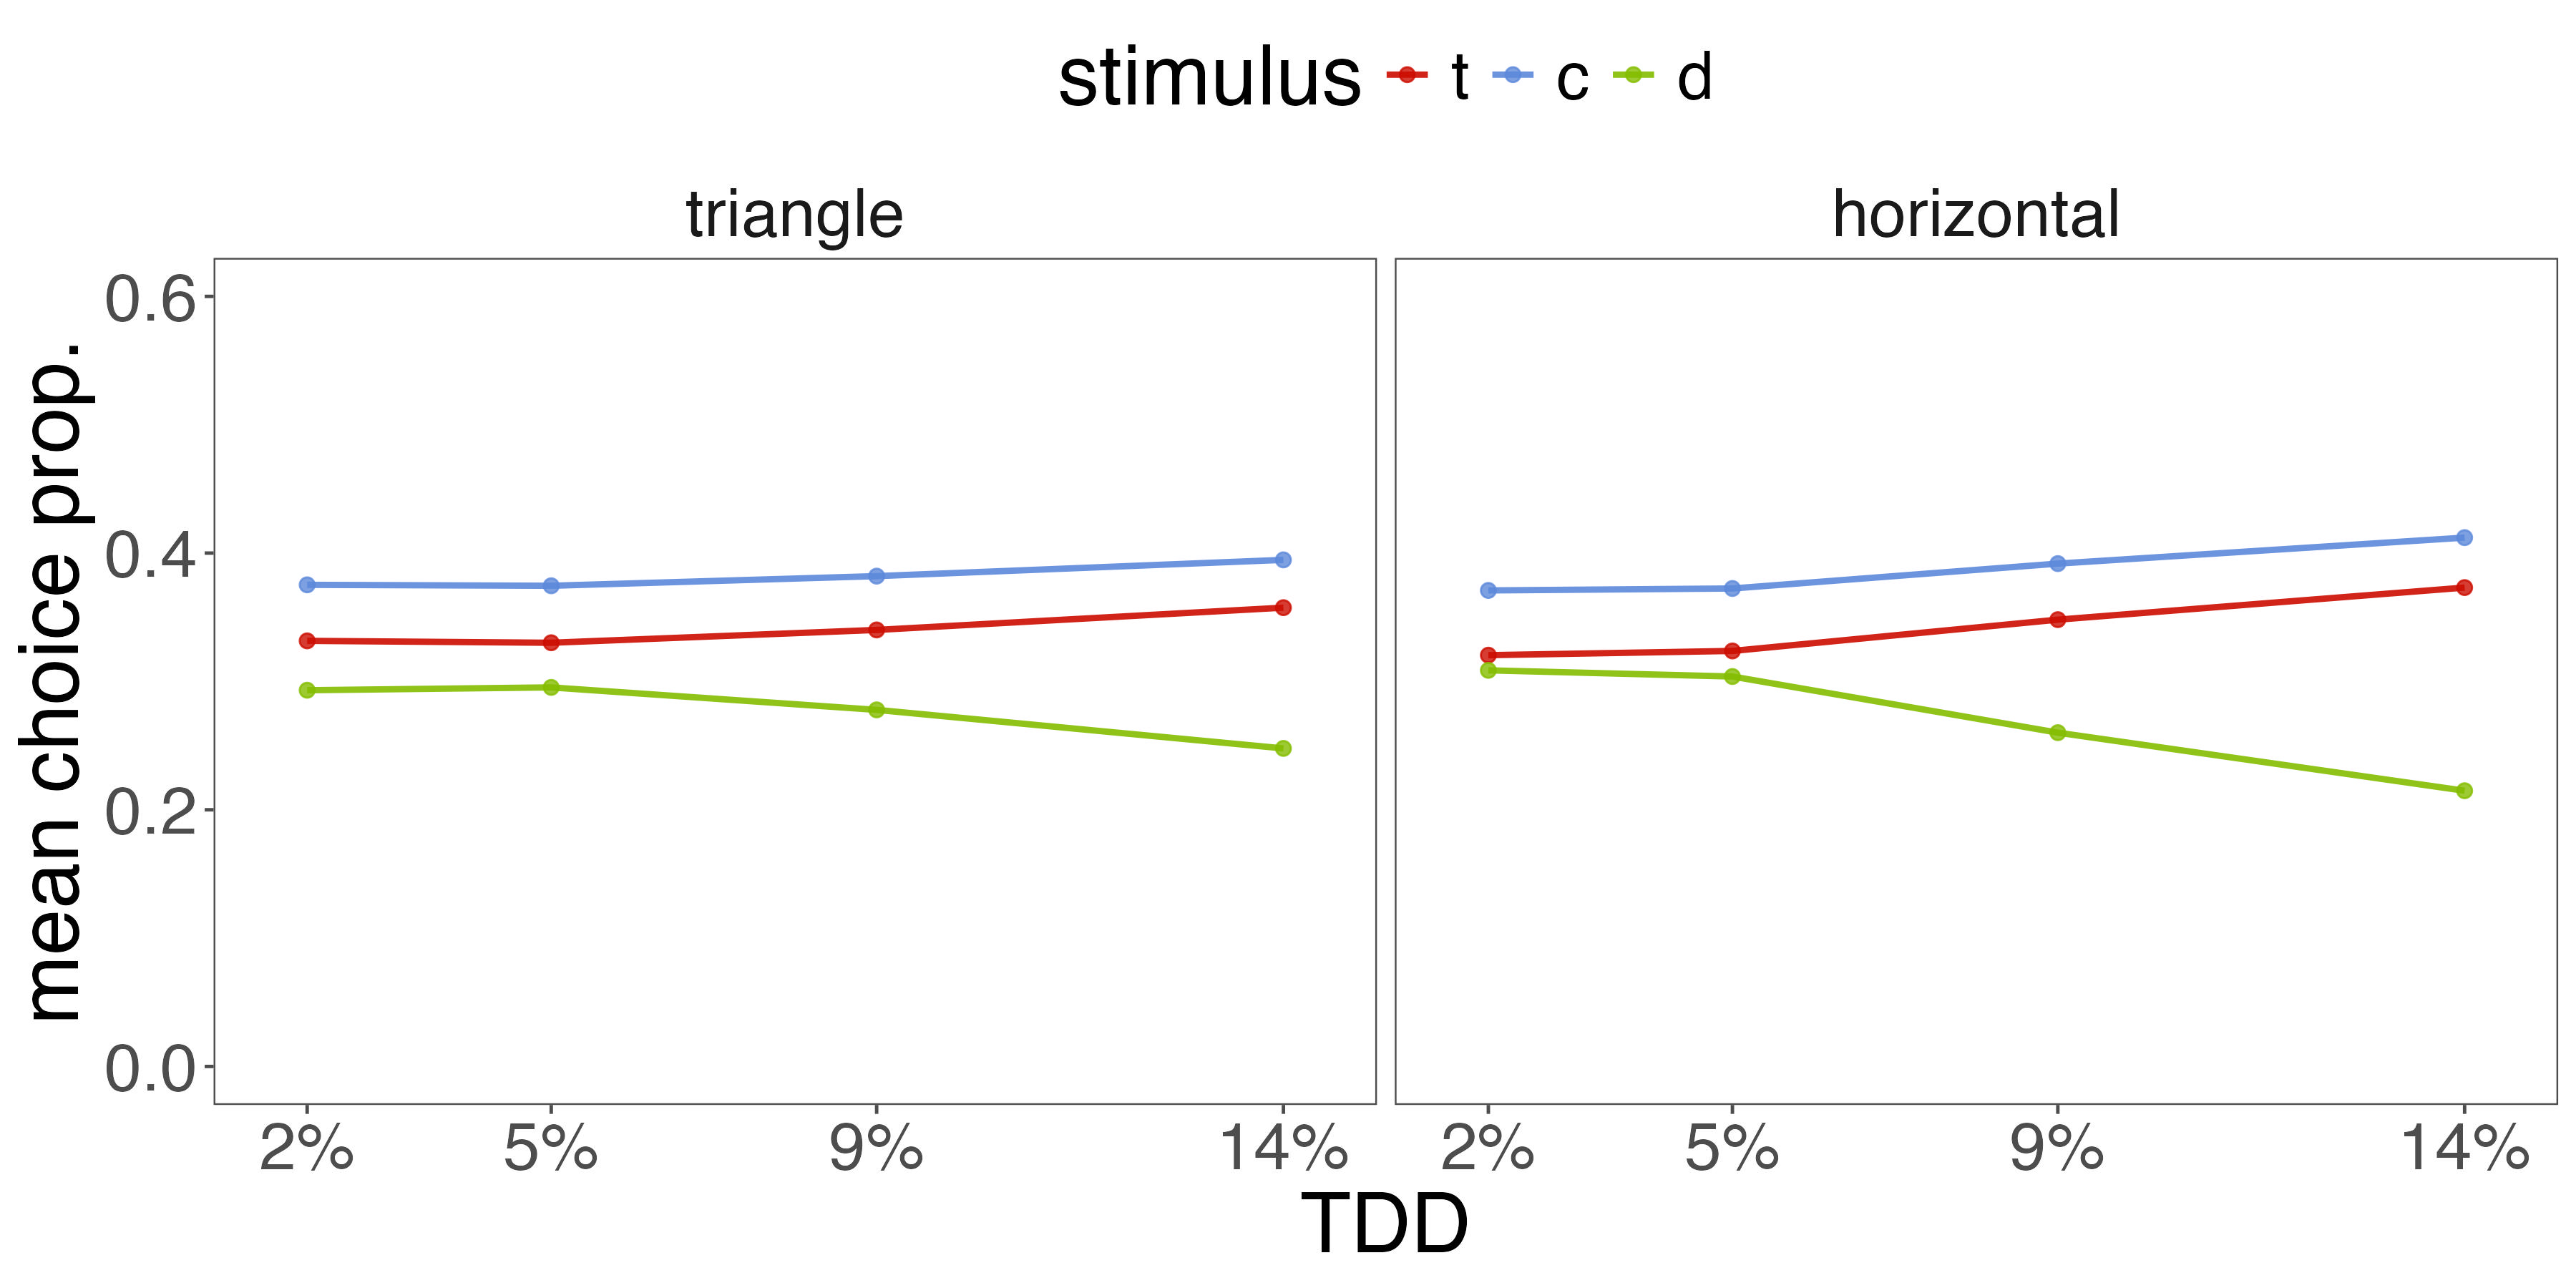
\includegraphics[width=\textwidth]{figures/bayes_circle_area_sim_choice_sigma_constant_comp_effect.jpeg}
   \caption{Model predictions for the choice data, conditioned on the mean estimated parameters from Experiment 2.}
   \label{fig:e2_model_preds}
\end{figure}

Conditioned on the estimated parameters, the model is able to produce a repulsion effect. This result aligns with our predictions; the repulsion effect, at least in some forms, can be generated by the Thurstonian perceptual choice model if the correlation between target and decoy perceptions is greater than the target-competitor and competitor-decoy correlations. In other words, the dependence between target and decoy perceptions is sufficient to produce the repulsion effect.

The model fails in predicting the null effect found at high TDD levels in the triangle condition, and it also fails completely in predicting the attraction effect. This is unsurprising, as to produce the attraction effect the model requires either $\mu_{T}>\mu_{C}$ or $\rho_{CD}>\rho_{TD}$, patterns not shown in the current parameter estimates. 

The model can produce the repulsion effect solely based on perceptual factors. That is, the model predicts the repulsion effect because the decoy is more likely to exceed the target in perceived area, than it is to exceed the competitor in perceived area.

Conditioned on the observed parameter estimates, the model cannot predict the attraction effect. Assuming the validity of the Thurstonian model, additional processes are needed to explain the attraction effect.

\section{Discussion}

The goal of Experiments 1 and 2 was to test the mechanisms generating the repulsion effect in perceptual choice. 

In Experiment 1, participants performed a two-alternative forced choice task, where on each trial they first saw a ternary set of target, competitor, and decoy rectangles before selecting the largest option from a particular pair (i.e., target/decoy, competitor/decoy, or target/competitor). The results showed that participants were not always able to discriminate between stimuli of differing areas (i.e., they selected the decoy a non-trivial proportion of the time). Furthermore, participants performed worse when the rectangles were arranged in the triangle display of \textcite{spektorWhenGoodLooks2018b} than in the horizontal display of \textcite{trueblood2013not}. Finally, participants were better at discriminating the target from the decoy than they were at discriminating the competitor from the decoy.

Experiment 2 was designed to estimate the parameters of a Thurstonian perceptual model and test the model's ability to predict the empirical results of a choice experiment. The experiment took place in two phases: a judgment phase, followed by a choice phase. On each trial in the judgment phase, participants saw a set of target, competitor, and decoy rectangles and estimated the areas of each rectangle by adjusting the size of corresponding circles. In each trial of the choice phase, participants saw three rectangles and were told to choose the rectangle with the largest area. The choice phase was a replication of \textcite{trueblood2013not} and \textcite{spektorWhenGoodLooks2018b}. 

The results of Experiments 1 and 2 show that participants are not always able to discriminate the decoy from the target and the competitor, and, that target-decoy perceptions are highly correlated. The observed correlations can, when embedded in a Thurstonian perceptual choice model, naturally produce the repulsion effect but not the attraction effect. This result is highly informative for decision-making research, as it shows to what extent the effects reported by \textcite{trueblood2013not} and \textcite{spektorWhenGoodLooks2018b} can be explained by valuation noise alone, and to what extent researchers must invoke higher-level decision processes to explain them. This finding does not rule out the possibility that the Thurstonian model is incorrect, but the model provides a parsimonious and empirically validated account of the repulsion effect.

To understand how these correlations produces the repulsion effect, consider the following simulation. 

First, two sets of parameters were generated. In each set, the $\boldsymbol{\mu}$ and $S$ values were similar to those estimated in Experiment 2, $\mu_{T}=\mu_{C}=0$, $\mu_{D}=-0.1$, $\sigma_{T}=\sigma_{C}=\sigma_{D}=\frac{1}{3}$. However, for the first set of parameters, all correlations were set equal, $\rho_{TC}=\rho_{CD}=\rho_{TD}=.75$, which were not observed in Experiment 2. For the second set of parameters, the correlations were set to comparable values from Experiment 2, $\rho_{TC}=\rho_{CD}=.65$, and $\rho_{TD}=.75$. 

Next, the Thurstonian model was simulated using each set of parameters. $1,000,000$ samples were drawn from the model (where, as above, a sample is a vector of target, competitor, and decoy perceived areas). For each sample, rankings were computed; for example, a ranking of TCD indicates that the target was perceived as largest, the competitor as second-largest, and the decoy as smallest. The simulation results are plotted in Figure~\ref{fig:sim_orderings}. 

\begin{figure}
   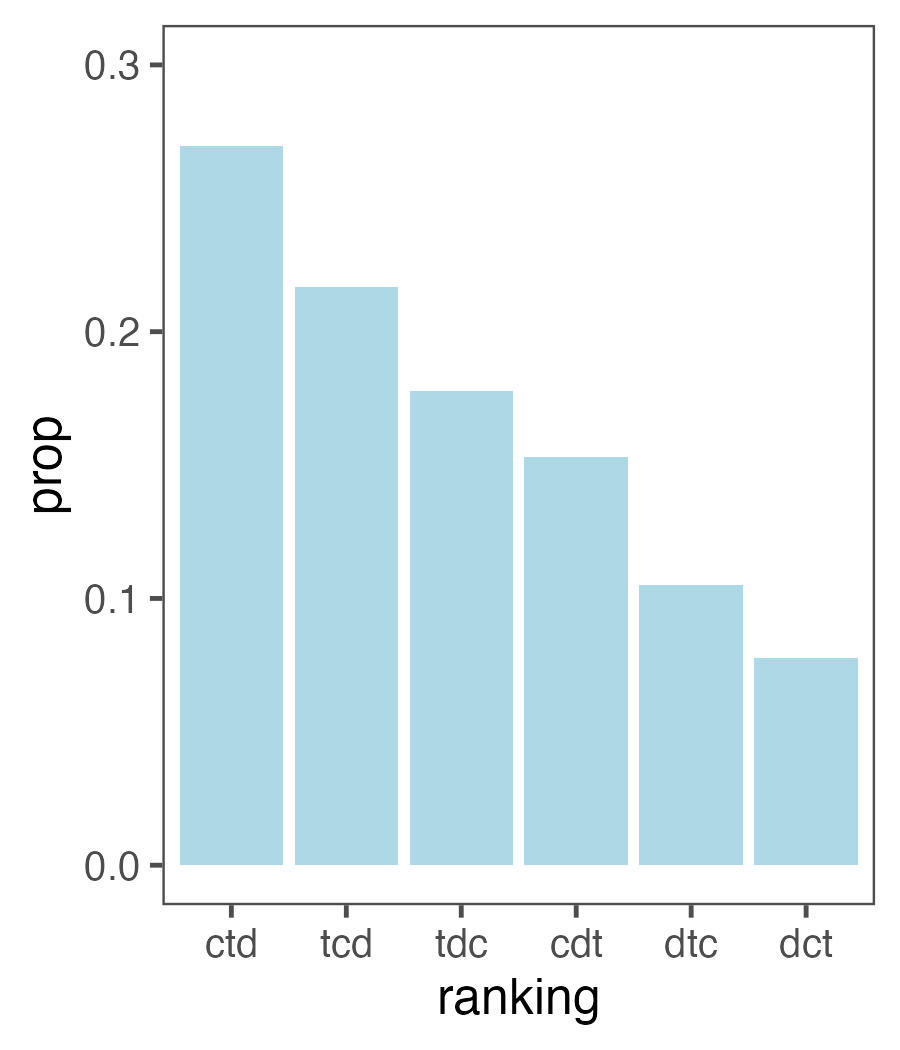
\includegraphics[width=100mm]{figures/sim_mvnorm_rank.jpeg}
   \caption{Model-simulated ranking proportions, in the order of largest to smallest.}
   \label{fig:sim_orderings}
\end{figure}

First, consider the parameter set where all correlations are equal (Figure~\ref{fig:sim_orderings}, top panel). The results show that $P(CTD)=P(TCD)>P(TDC)=P(CDT)>P(DTC)=P(DCT)$. The decoy is most likely be perceived smallest, least likely to be perceived largest, and the perceived size of the decoy does not influence the relative perception of target and competitor; The target and competitor are equally likely to be perceived as largest (e.g., $P(CTD)=P(TCD)$).

Now consider the parameter set where $\rho_{TD}>\rho_{TC}=\rho_{CD}$ (Figure~\ref{fig:sim_orderings}, bottom panel). Here, $P(CTD)>P(TCD)$, because the target and decoy tend to move together, making it easier for the competitor to exceed both options. Furthermore, $P(DTC)>P(DCT)$, because the relatively large $\rho_{TD}$ also allows the decoy to be pulled up with the target. These correlations also cause $P(TDC)>P(CDT)$. In simple terms, if the decoy is in the middle, it is more likely that the target is the largest than it is that the competitor is largest. Note that if we sum up these orderings we can obtain the marginal choice proportions for $T$, $C$, and $D$ which will show a repulsion effect, i.e., $P(C)>P(T)>P(D)$. 

Thus far the research provides a statistical account of these data, but a process account is (one) ultimate goal of cognitive psychology research. I argue that the target and decoy, which are inherently more similar to one another than either is to the competitor, are more likely to be compared to one another. This ease of comparison leads to correlated valuations which in turn affects choice. This account is plausible based both on this research and on prior decision-making research.

Other researchers have suggested that correlated valuations may be a measure of similarity between choice options. \textcite{kamakura1984predicting} and \textcite{natenzon2019random} both estimated correlations indirectly from choice data, by applying constraints to variants of the multinomial probit model. The current research is, to the author's knowledge, the first to directly estimate these correlations through trial-level valuations. 

Multialternative Decision Field Theory (MDFT) \parencite{roeMultialternativeDecisionField2001a} relies on within-trial correlations between similar options to produce the similarity effect, though this mechanism is distinct from the current model, which relies on \textit{across-trial} correlated valuations. 

\textcite{bhui2021rational} showed that target and decoy valuations may be correlated, and they further argued that the repulsion effect is rational given a consumer's belief that the target and decoy come from the same distribution (e.g., two products from the same brand). \textcite{bhui2024context} similarly argued that context effects can be rational given limited information about options in a choice set. 

The results of Experiments 1 and 2 have important methodological implications. \textcite{trueblood2013not} and \textcite{spektorWhenGoodLooks2018b} designed their studies to test the interesting hypothesis that context effects occur even in low-level, perceptual decision-making. They designed experiments similar to other attraction effect experiments, with two equally viable focal options and an inferior decoy option which is similar to a focal target option. While acknowledging that participants may occasionally fail to perceive the dominance relationship, \textcite{spektorWhenGoodLooks2018b} dismissed the possibility that their repulsion effect may be a form of the \textit{similarity effect}, where two similar options split choice shares, but they dismissed this hypothesis because participants chose the target more often than they chose the decoy. They did not consider the possibility, however, that the target-decoy comparability could cause perceptual correlations which manifest themselves in the choice data.  Experiment 2 showed that, even though $P(T)>P(D)$, the decoy is systematically chosen over the target more than it is chosen over the competitor. Thus, the correlation between target and decoy can generate a repulsion effect that is qualitatively different from a reversal of the attraction effect.

Researchers have also argued in favor of the "tainting hypothesis" \parencite{simonson2014vices,spektorWhenGoodLooks2018b}, where the inferior decoy "taints" similar options (i.e., the target). On average, participants did generally rate the competitor as larger than the target in Experiment 2. These results were, however, quite small and not always statistically apparent. Moreover, the model does not require this tainting to produce the repulsion effect.

Researchers should be careful in assuming that an empirical context effect is generated solely by decision processes whenever the choice environment precludes full stimulus discriminability. Though data from \textcite{spektorWhenGoodLooks2018b} showed an empirical repulsion effect (i.e., competitor chosen less than the competitor), this chapter has presented evidence that the data are generated from a fundamentally different process than the attraction effect. 

There are some limitations to the current experiment. Due to the large amount of data required to estimate a variance-covariance matrix \parencite{martin2021,merkle2023opaque}, The correlation parameters were estimated by collapsing across participants. The aggregation of data may obscure individual differences, an area of increasing concern in context effect research \parencite{liewAppropriacyAveragingStudy2016b,trueblood2015fragile,davis2023illustrated}. Future studies  should collect enough participant-level data (perhaps by asking participants to return for multiple experimental sessions) to allow participant-level variation in correlation estimates. It would be of great theoretical interest if individual differences in the correlation parameters could explain individual variation in the attraction and repulsion effects. If the repulsion effect in perceptual choice is truly generated by target-decoy similarity, then, at an individual participant level, the strength of the repulsion effect should be positively related to the value of $\rho_{TD}$. Participants who are more prone to confusing target and decoy should show a stronger repulsion effect.

Participants also appeared to use both relative and absolute judgment processes when judging the areas of the rectangles. Mean judgments of decoy sized decreased with TDD, but mean target and competitor judgments decreased as well. Thus, the measurements of area perception are not ideal, though these measurements were sufficient for the current purposes. 

As discussed in the Appendix, there was a wide bias during the choice phase but a tall bias during the judgment phase. In the choice phase, participants chose wide rectangles more than tall rectangles. In the judgment phase, however, they judged tall rectangles to be larger than wide (at least in the triangle condition). The latter effect is quite small (i.e., smaller than that of the difference between the target and the smallest decoy), but it is nonetheless present in the data. There is currently no clear explanation for this result. \textcite{gronau2023choice} compared participants' ability to perform a perceptual discrimination task based on whether they responded via an ordinal rating scale or a choice. The authors concluded that participants relied on the same representation in both cases, but the participants were more sensitive to stimulus-level differences when choice responses were collected. It may be that, in Experiment 2, the relative lack of perceptual sensitivity caused participants to slightly underestimate their reported responses to stimuli they actually \textit{perceived} as larger. This inconsistency may also be idiosyncratic statistical variation which may not appear in future samples. 

This chapter shows that the repulsion effect in perceptual choice can be explained by target-decoy similarity alone, but the attraction effect may require invoking higher-level decision processes. To explain the repulsion effect, a Thurstonian perceptual choice model was developed and tested. In particular, the means, variances, and correlations of multivariate Gaussian distribution of area perception were jointly estimated from participants' judgments of perceptual stimuli. This model was then tested on its ability to explain choice data collected from the same participants. This research furthers the study of context effects, provides a new experimental paradigm for testing them, and helps explain inconsistencies in prior results.
